\mfpicnumber{1}

\opengraphsfile{TrigGraphs}

\setcounter{footnote}{0}

\label{TrigGraphs}

In this section, we return to our discussion of the circular (trigonometric) functions as functions of real numbers and pick up where we left off in Sections \ref{cosinesinebeyond} and \ref{circularfunctionsbeyond}.  As usual, we begin our study with the functions $f(t) = \cos(t)$ and $g(t) = \sin(t)$.  

\subsection{Graphs of the Cosine and Sine Functions}

From Theorem \ref{cosinesinefunctiondomainrange} in Section \ref{cosinesinebeyond}, we know that the domain of $f(t) = \cos(t)$ and of $g(t) = \sin(t)$ is all real numbers, $(-\infty, \infty),$ and the range of both functions is $[-1,1]$.  The Even / Odd Identities in Theorem \ref{evenodd} tell us $\cos(-t) = \cos(t)$ for all real numbers $t$ and $\sin(-t) = -\sin(t)$ for all real numbers $t$.  This means $f(t) = \cos(t)$ is an even function, while $g(t) = \sin(t)$ is an odd function.\footnote{See section \ref{GraphsofFunctions} for a review of these concepts.}  Another important property of these  functions is that for coterminal angles $\alpha$ and $\beta$, $\cos(\alpha) = \cos(\beta)$ and $\sin(\alpha) = \sin(\beta)$.  Said differently,  $\cos(t + 2\pi k) = \cos(t)$ and $\sin(t + 2\pi k) = \sin(t)$ for all real numbers $t$ and any integer $k$.  This last property is given a special name.

\smallskip

\colorbox{ResultColor}{\bbm

\begin{defn} \label{periodic} \textbf{Periodic Functions:} A function $f$ is said to be \textbf{periodic}\index{function ! periodic}\index{periodic function}  if there is a real number $c$ so that $f(t+c) = f(t)$ for all real numbers $t$ in the domain of $f$.  The smallest positive number $p$ for which $f(t+p) = f(t)$ for all real numbers $t$ in the domain of $f$, if it exists, is called the \textbf{period} of $f$. \index{period ! of a function}

\end{defn}

\ebm}

\medskip

We have already seen a family of periodic functions in Section \ref{LinearFunctions}:  the constant functions.  However, despite being periodic a constant function has no period.  (We'll leave that odd gem as an exercise for you.)  Returning to the circular functions, we see that by Definition \ref{periodic}, $f(t) = \cos(t)$ is periodic, since $\cos(t + 2\pi k) = \cos(t)$ for any integer $k$.  To determine the period of $f$, we need to find the smallest real number $p$ so that $f(t+p) = f(t)$ for all real numbers $t$ or, said differently, the smallest positive real number $p$ such that $\cos(t+p) = \cos(t)$  for all real numbers $t$.  We know that $\cos(t + 2\pi) = \cos(t)$ for all real numbers $t$ but the question remains if any smaller real number will do the trick.  Suppose $p>0$ and $\cos(t + p) = \cos(t)$ for all real numbers $t$.  Then, in particular, $\cos(0+p) = \cos(0)$ so that $\cos(p) = 1$.  From this we know $p$ is a multiple of $2\pi$ and, since the smallest positive multiple of $2\pi$ is $2\pi$ itself, we have the result.  Similarly, we can show $g(t) = \sin(t)$ is also periodic with $2\pi$ as its period.\footnote{Alternatively,  we can use the Cofunction Identities in Theorem \ref{cofunctionidentities} to show that $g(t) = \sin(t)$ is periodic with period $2\pi$ since $g(t) = \sin(t) = \cos\left(\frac{\pi}{2} - t\right) = f\left(\frac{\pi}{2} - t\right)$.}  Having period $2\pi$ essentially means that we can completely understand everything about the functions  $f(t) = \cos(t)$ and $g(t) = \sin(t)$ by studying one interval of length $2\pi$, say $[0,2\pi]$.\footnote{Technically, we should study the interval $[0,2\pi)$,\footnotemark since whatever happens at $t=2\pi$ is the same as what happens at $t=0$.  As we will see shortly, $t=2\pi$ gives us an extra `check' when we go to graph these functions.} \footnotetext{In some advanced texts, the interval of choice is $[-\pi, \pi)$.} 

\smallskip

One last property of the functions $f(t) = \cos(t)$ and $g(t) = \sin(t)$ is worth pointing out:   both of these functions are continuous and smooth.  Recall from Section \ref{GraphsofPolynomials} that geometrically this means the graphs of the cosine and sine functions have no jumps, gaps, holes in the graph,  asymptotes, corners or cusps.  As we shall see, the graphs of both $f(t) = \cos(t)$ and $g(t) = \sin(t)$ meander nicely and don't cause any trouble.  We summarize these facts in the following theorem.


\smallskip

\colorbox{ResultColor}{\bbm

\begin{thm} \label{cosinesinefunctionprops}  \textbf{Properties of the Cosine and Sine Functions} \index{cosine ! properties of} \index{sine ! properties of}

\vspace{.2in}

\begin{tabular}{ll}

\hspace{.3in} $\bullet \, $ The function $f(x) = \cos(x)$ & \hspace{.8in} $\bullet \, $ The function $g(x) = \sin(x)$ \\
  & \\

\hspace{.5in} -- has domain $(-\infty, \infty)$ & \hspace{1in} -- has domain $(-\infty, \infty)$ \\ [4pt]
\hspace{.5in} -- has range $[-1,1]$ & \hspace{1in} -- has range $[-1,1]$ \\ [4pt]
\hspace{.5in} -- is continuous and smooth & \hspace{1in} -- is continuous and smooth \\ [4pt]
\hspace{.5in} -- is even & \hspace{1in} -- is odd \\ [4pt]
\hspace{.5in} -- has period $2\pi$ & \hspace{1in} -- has period $2\pi$ \\ 

\end{tabular}

\end{thm}

\ebm}

\medskip

In the chart above, we followed the convention established in Section \ref{GraphsofFunctions} and used $x$ as the independent variable and $y$ as the dependent variable.\footnote{The use of $x$ and $y$ in this context is not to be confused with the $x$- and $y$-coordinates of points on the Unit Circle which define cosine and sine.  Using the term `trigonometric function' as opposed to `circular function' can help with that, but one could then ask, ``Hey, where's the triangle?''}  This allows us to turn our attention to graphing the cosine and sine functions in the Cartesian Plane.  To graph $y = \cos(x)$, we make a table as we did in Section \ref{GraphsofFunctions} using some of the `common values' of $x$ in the interval $[0,2\pi]$. This generates a \textit{portion} of the cosine graph, which we call the \index{fundamental cycle ! of $y = \cos(x)$}`\textbf{fundamental cycle}' of $y = \cos(x)$. \index{cosine ! graph of}

\hspace{.5in} \begin{tabular}{m{2.7in}m{3in}}
\setlength{\extrarowheight}{2pt}
\[ \begin{array}{|r||r|r|}  

\hline

 x & \cos(x) & (x,\cos(x)) \\ \hline
0  & 1 & (0, 1) \\ [2pt]   \hline
\frac{\pi}{4}  & \frac{\sqrt{2}}{2} & \left(\frac{\pi}{4}, \frac{\sqrt{2}}{2}\right) \\ [2pt] \hline 
\frac{\pi}{2}  & 0 & \left(\frac{\pi}{2}, 0\right) \\ [2pt] \hline 
\frac{3\pi}{4}  & -\frac{\sqrt{2}}{2} & \left(\frac{3\pi}{4}, -\frac{\sqrt{2}}{2}\right) \\ [2pt] \hline 
\pi & -1 & (\pi, -1) \\ [2pt] \hline 
\frac{5\pi}{4}  & -\frac{\sqrt{2}}{2} & \left(\frac{5\pi}{4}, -\frac{\sqrt{2}}{2}\right) \\ [2pt] \hline 
\frac{3\pi}{2}  & 0 & \left(\frac{3\pi}{2}, 0 \right) \\ [2pt] \hline 
\frac{7\pi}{4}  & \frac{\sqrt{2}}{2} & \left(\frac{7\pi}{4}, \frac{\sqrt{2}}{2}\right) \\ [2pt] \hline 
2\pi  & 1 & (2\pi, 1) \\  [2pt] \hline
\end{array} \] \setlength{\extrarowheight}{0pt} &

\begin{mfpic}[25][50]{-1}{7}{-1.5}{1.5}
\point[3pt]{(0,1), (0.7854,0.7071), (1.5708,0), (2.3562,-0.7071), (3.1416, -1), (3.9270,-0.7071), (4.7124,0), (5.4978,0.7071), (6.2832,1)}
\axes
\tlabel[cc](7,-0.15){\scriptsize $x$}
\tlabel[cc](0.25,1.5){\scriptsize $y$}
\tcaption{The `fundamental cycle' of $y = \cos(x)$.}
\xmarks{0.7854, 1.5708, 2.3562, 3.1416, 3.9270, 4.7124,5.4978,6.2832 }
\ymarks{-1,1}
\tlpointsep{4pt}
\scriptsize
\axislabels {x}{{$\frac{\pi}{4}$} 0.7854, {$\frac{\pi}{2}$} 1.5708, {$\frac{3\pi}{4}$} 2.3562, {$\pi$} 3.1416, {$\frac{5\pi}{4}$} 3.9270, {$\frac{3\pi}{2}$} 4.7124, {$\frac{7\pi}{4}$} 5.4978, {$2\pi$} 6.2832}
\normalsize
\axislabels {y}{{\scriptsize $-1$} -1, {\scriptsize $1$} 1}
\function{0, 6.2832, 0.1}{cos(x)}
\end{mfpic} \\

\end{tabular}

A few things about the graph above are worth mentioning. First, this graph represents only part of the graph of $y = \cos(x)$.  To get the entire graph, we imagine `copying and pasting' this graph end to end infinitely in both directions (left and right) on the $x$-axis.  Secondly, the vertical scale here has been greatly exaggerated for clarity and aesthetics. Below is an accurate-to-scale graph of $y = \cos(x)$ showing several cycles with the `fundamental cycle' plotted thicker than the others.    The graph of $y=\cos(x)$ is usually described as `wavelike' -- indeed, many of the applications involving the cosine and sine functions feature modeling wavelike phenomena.   

\begin{center}

\begin{mfpic}[15]{-13}{13}{-1.5}{1.5}
\axes
\point[3pt]{(0,1), (6.2832,1)}
\tlabel[cc](13,-0.5){\scriptsize $x$}
\tlabel[cc](0.5,1.5){\scriptsize $y$}
\tcaption{An accurately scaled graph of $y = \cos(x)$.}
\ymarks{-1,1}
\arrow \reverse \arrow \function{-12.5664, 12.5664, 0.1}{cos(x)}
\penwd{1.5pt}
\function{0, 6.2832, 0.1}{cos(x)}
\end{mfpic}

\end{center} 

We can plot the fundamental cycle of the graph of $y = \sin(x)$ similarly, with similar results.  \index{sine ! graph of}

\hspace{.5in} \begin{tabular}{m{2.7in}m{3in}}
\setlength{\extrarowheight}{2pt}
\[ \begin{array}{|r||r|r|}  

\hline

 x & \sin(x) & (x,\sin(x)) \\ \hline
0  & 0 & (0, 0) \\ [2pt]   \hline
\frac{\pi}{4}  & \frac{\sqrt{2}}{2} & \left(\frac{\pi}{4}, \frac{\sqrt{2}}{2}\right) \\ [2pt] \hline 
\frac{\pi}{2}  & 1 & \left(\frac{\pi}{2}, 1\right) \\ [2pt] \hline 
\frac{3\pi}{4}  & \frac{\sqrt{2}}{2} & \left(\frac{3\pi}{4}, \frac{\sqrt{2}}{2}\right) \\ [2pt] \hline 
\pi & 0 & (\pi, 0) \\ [2pt] \hline 
\frac{5\pi}{4}  & -\frac{\sqrt{2}}{2} & \left(\frac{5\pi}{4}, -\frac{\sqrt{2}}{2}\right) \\ [2pt] \hline 
\frac{3\pi}{2}  & -1 & \left(\frac{3\pi}{2}, -1 \right) \\ [2pt] \hline 
\frac{7\pi}{4}  & -\frac{\sqrt{2}}{2} & \left(\frac{7\pi}{4}, -\frac{\sqrt{2}}{2}\right) \\ [2pt] \hline 
2\pi  & 0 & (2\pi, 0) \\  [2pt] \hline
\end{array} \] \setlength{\extrarowheight}{0pt} &

\begin{mfpic}[25][50]{-1}{7}{-1.5}{1.5}
\point[3pt]{(0,0), (0.7854,0.7071), (1.5708,1), (2.3562,0.7071), (3.1416, 0), (3.9270,-0.7071), (4.7124,-1), (5.4978,-0.7071), (6.2832,0)}
\axes
\tlabel[cc](7,-0.15){\scriptsize $x$}
\tlabel[cc](0.25,1.5){\scriptsize $y$}
\tcaption{The `fundamental cycle' of $y = \sin(x)$.}
\xmarks{0.7854, 1.5708, 2.3562, 3.1416, 3.9270, 4.7124,5.4978,6.2832 }
\ymarks{-1,1}
\tlpointsep{4pt}
\scriptsize
\axislabels {x}{{$\frac{\pi}{4}$} 0.7854, {$\frac{\pi}{2}$} 1.5708, {$\frac{3\pi}{4}$} 2.3562, {$\pi$} 3.1416, {$\frac{5\pi}{4}$} 3.9270, {$\frac{3\pi}{2}$} 4.7124, {$\frac{7\pi}{4}$} 5.4978, {$2\pi$} 6.2832}
\normalsize
\axislabels {y}{{\scriptsize $-1$} -1, {\scriptsize $1$} 1}
\function{0, 6.2832, 0.1}{sin(x)}
\end{mfpic} \\

\end{tabular}

As with the graph of $y=\cos(x)$, we provide an accurately scaled graph of $y = \sin(x)$ below with the fundamental cycle highlighted.

\begin{center}

\begin{mfpic}[15]{-13}{13}{-1.5}{1.5}
\axes
\point[3pt]{(0,0), (6.2832,0)}
\tlabel[cc](13,-0.5){\scriptsize $x$}
\tlabel[cc](0.5,1.5){\scriptsize $y$}
\tcaption{An accurately scaled graph of $y = \sin(x)$.}
\ymarks{-1,1}
\arrow \reverse \arrow \function{-12, 12, 0.1}{sin(x)}
\penwd{1.5pt}
\function{0, 6.2832, 0.1}{sin(x)}
\end{mfpic}

\end{center} 

It is no accident that the graphs of $y = \cos(x)$ and $y = \sin(x)$ are so similar.  Using a cofunction identity along with the even property of cosine, we have

\[ \sin(x) = \cos\left(\frac{\pi}{2} - x\right) = \cos\left(-\left(x - \frac{\pi}{2}\right)\right) = \cos\left(x - \frac{\pi}{2}\right)\]

Recalling Section \ref{Transformations}, we see from this formula that the graph of $y=\sin(x)$ is the result of shifting the graph of $y = \cos(x)$ to the right $\frac{\pi}{2}$ units.  A visual inspection confirms this. 

\smallskip

Now that we know the basic shapes of the graphs of $y = \cos(x)$ and $y = \sin(x)$, we can use Theorem \ref{transformationsthm} in Section \ref{Transformations} to graph more complicated curves.  To do so, we need to keep track of the movement of some key points on the original graphs. We choose to track the values $x = 0$, $\frac{\pi}{2}$, $\pi$, $\frac{3\pi}{2}$ and $2\pi$.  These `quarter marks' correspond to quadrantal angles, and as such, mark the location of the zeros and the local extrema of these functions over exactly one period.  Before we begin our next example, we need to review the concept of the `argument' of a function as first introduced in Section \ref{FunctionNotation}.  For the function $f(x) = 1 - 5\cos(2x-\pi)$, the argument of $f$ is $x$.  We shall have occasion, however, to refer to the argument of the \textit{cosine}, which in this case is $2x-\pi$.  Loosely stated, the argument of a trigonometric function is the expression `inside' the function.\index{argument ! of a trigonometric function}

\begin{ex}  \label{cosinesinegraphex1} Graph one cycle of the following functions. State the period of each.

\begin{multicols}{2}

\begin{enumerate}

\item  $f(x) = 3 \cos\left(\frac{\pi x - \pi}{2}\right) + 1$

\item  $g(x) = \frac{1}{2} \sin(\pi - 2x) + \frac{3}{2}$

\end{enumerate}

\end{multicols}

{\bf Solution.}

\begin{enumerate}

\item  We set the argument of the cosine, $\frac{\pi x - \pi}{2}$, equal to each of the values:  $0$, $\frac{\pi}{2}$, $\pi$, $\frac{3\pi}{2}$, $2\pi$ and solve for $x$. We summarize the results below.
\setlength{\extrarowheight}{2pt}
\[ \begin{array}{|r|r|r|}  

\hline

 a & \frac{\pi x - \pi}{2} = a & x \\ [2pt] \hline

0  & \frac{\pi x - \pi}{2} = 0 & 1 \\ [2pt]   \hline

\frac{\pi}{2}  & \frac{\pi x - \pi}{2} = \frac{\pi}{2} & 2 \\ [2pt] \hline 

\pi & \frac{\pi x - \pi}{2} = \pi & 3 \\ [2pt] \hline 

\frac{3\pi}{2}  & \frac{\pi x - \pi}{2} = \frac{3\pi}{2} & 4 \\ [2pt] \hline 

2\pi  & \frac{\pi x - \pi}{2} = 2\pi & 5\\  [2pt] \hline
\end{array} \]
\setlength{\extrarowheight}{0pt}

Next, we substitute each of these $x$ values into $f(x) = 3 \cos\left(\frac{\pi x - \pi}{2}\right) + 1$ to determine the corresponding $y$-values and connect the dots in a pleasing wavelike fashion. 


\hspace{.5in} \begin{tabular}{m{2.7in}m{3in}}
\setlength{\extrarowheight}{2pt}
\setlength{\extrarowheight}{2pt}
\[ \begin{array}{|r||r|r|}  

\hline

 x & f(x) & (x,f(x)) \\ [2pt] \hline
1  & 4 & (1,4) \\ [2pt]   \hline

2  & 1 & (2,1) \\ [2pt] \hline 

3 & -2 & (3,-2) \\ [2pt] \hline 

4  & 1 & (4,1) \\ [2pt] \hline 

5 & 4 & (5,4) \\  [2pt] \hline
\end{array} \]
\setlength{\extrarowheight}{0pt} &

\begin{mfpic}[15]{-1}{6}{-3}{5}
\point[3pt]{(1,4), (2,1), (3,-2), (4,1), (5, 4)}
\axes
\tlabel[cc](6,-0.25){\scriptsize $x$}
\tlabel[cc](0.25,5){\scriptsize $y$}
\tcaption{\scriptsize One cycle  of $y = f(x)$.}
\xmarks{1,2,3,4,5}
\ymarks{-2,-1,1,2,3,4}
\tlpointsep{4pt}
\axislabels {x}{{\tiny $1$} 1, {\tiny $2$} 2, {\tiny $3$} 3, {\tiny $4$} 4, {\tiny $5$} 5}
\axislabels {y}{{\tiny $-2$} -2,{\tiny $-1$} -1, {\tiny $1$} 1, {\tiny $2$} 2, {\tiny $3$} 3, {\tiny $4$} 4}
\function{1, 5, 0.1}{3*cos((3.14159*x - 3.14159)/2)+1}
\end{mfpic} \\

\end{tabular}

One cycle is graphed on $[1,5]$ so the period is the length of that interval which is $4$.

\item  Proceeding as above, we set the argument of the sine, $\pi - 2x$, equal to each of our quarter marks and solve for $x$.

\setlength{\extrarowheight}{2pt}
\[ \begin{array}{|r|r|r|}  

\hline

 a & \pi - 2x = a & x \\ [2pt] \hline
0  & \pi - 2x = 0 & \frac{\pi}{2} \\ [2pt]   \hline

\frac{\pi}{2}  &\pi - 2x = \frac{\pi}{2} & \frac{\pi}{4} \\ [2pt] \hline 

\pi & \pi - 2x = \pi & 0 \\ [2pt] \hline 

\frac{3\pi}{2}  & \pi - 2x = \frac{3\pi}{2} & -\frac{\pi}{4} \\ [2pt] \hline 

2\pi  &\pi - 2x = 2\pi & -\frac{\pi}{2}\\  [2pt] \hline
\end{array} \]
\setlength{\extrarowheight}{0pt}

We now find the corresponding $y$-values on the graph by substituting each of these $x$-values into  $g(x) = \frac{1}{2} \sin(\pi - 2x) + \frac{3}{2}$.  Once again, we connect the dots in a wavelike fashion.

\hspace{.5in} \begin{tabular}{m{2.7in}m{3in}}
\setlength{\extrarowheight}{2pt}
\setlength{\extrarowheight}{2pt}
\[ \begin{array}{|r||r|r|}  

\hline

 x & g(x) & (x,g(x)) \\ [2pt] \hline
\frac{\pi}{2} & \frac{3}{2} & \left(\frac{\pi}{2}, \frac{3}{2}\right)  \\ [2pt]   \hline

\frac{\pi}{4} & 2 & \left(\frac{\pi}{4}, 2\right) \\ [2pt] \hline 

0 & \frac{3}{2} & \left(0, \frac{3}{2} \right)  \\ [2pt] \hline 

-\frac{\pi}{4}  & 1 &  \left(-\frac{\pi}{4}, 1 \right) \\ [2pt] \hline 

-\frac{\pi}{2} & \frac{3}{2} & \left(-\frac{\pi}{2}, \frac{3}{2} \right) \\  [2pt] \hline
\end{array} \]
\setlength{\extrarowheight}{0pt} &

\begin{mfpic}[25]{-2}{2}{0}{3}

\point[3pt]{(1.5708,1.5), (0.7854,2), (0,1.5), (-0.7854,1), (-1.5708,1.5)}
\axes
\tlabel[cc](2,-0.25){\scriptsize $x$}
\tlabel[cc](0.25,3){\scriptsize $y$}
\tcaption{\scriptsize One cycle  of $y = g(x)$.}
\xmarks{-1.5708,-0.7854,0.7854,1.5708}
\ymarks{1,2}
\tlpointsep{4pt}
\axislabels {x}{{\tiny $-\dfrac{\pi}{2} \hspace{7pt}$} -1.5708, {\tiny $-\dfrac{\pi}{4}\hspace{7pt}$} -0.7854, {\tiny $\dfrac{\pi}{4}$} 0.7854,  {\tiny $\dfrac{\pi}{2}$} 1.5708}
\axislabels {y}{ {\tiny $1$} 1, {\tiny $2$} 2}
\function{-1.5708, 1.5708, 0.1}{0.5*sin(3.14159-2*x)+1.5}
\end{mfpic} \\

\end{tabular}

One cycle was graphed on the interval $\left[ -\frac{\pi}{2}, \frac{\pi}{2}\right]$ so the period is $\frac{\pi}{2} - \left(-\frac{\pi}{2}\right) = \pi$. \qed

\end{enumerate}

\end{ex}

The functions in Example \ref{cosinesinegraphex1} are examples of \textbf{sinusoids}. Roughly speaking, a sinusoid is the result of taking the basic graph of $f(x) = \cos(x)$ or $g(x) = \sin(x)$ and performing any of the transformations\footnote{We have already seen how the Even/Odd and Cofunction Identities can be used to rewrite $g(x) = \sin(x)$ as a transformed version of $f(x) = \cos(x)$, so of course, the reverse is true:  $f(x) = \cos(x)$ can be written as a transformed version of $g(x) = \sin(x)$.  The authors have seen some instances where sinusoids are always converted to cosine functions while in other disciplines, the sinusoids are always written in terms of sine functions.  We will discuss the applications of sinusoids in greater detail in Chapter \ref{AppExt}.  Until then, we will keep our options open.} mentioned in Section \ref{Transformations}.  Sinusoids can be characterized by four properties:  period, amplitude, phase shift and vertical shift. We have already discussed period, that is, how long it takes for the sinusoid to complete one cycle.  The standard period of both $f(x) = \cos(x)$ and $g(x) = \sin(x)$ is $2\pi$, but horizontal scalings will change the period of the resulting sinusoid.  The \index{amplitude}\index{sinusoid ! amplitude}\textbf{amplitude} of the sinusoid is a measure of how `tall' the wave is, as indicated in the figure below.  The amplitude of the standard cosine and sine functions is $1$, but vertical scalings can alter this.  
\begin{center}

\begin{mfpic}[15]{-6.5}{6.5}{-6.5}{6.5}
\dashed \polyline{(-6.2832,0), (6.2832,0)}
\function{-6.2832, 6.2832, 0.1}{0-6*sin(x/2)}
\arrow \reverse \arrow \polyline{(-3.1416, 0.25), (-3.1416, 5.75)}
\gclear \tlabelrect[cc](-3.1416, 3){amplitude}
\gclear \tlabelrect[cc](3.1416, 0){baseline}
\arrow \reverse \arrow \polyline{(-6.2832,-6.5), (6.2832,-6.5)}
\gclear \tlabelrect[cc](0, -6.5){period}
\end{mfpic}

\end{center}

\vspace{-.05in}

The \index{phase shift}\index{sinusoid ! phase shift}\textbf{phase shift} of the sinusoid is the horizontal shift experienced by the fundamental cycle.\index{sinusoid ! graph of} We have seen that a phase (horizontal) shift of $\frac{\pi}{2}$ to the right takes $f(x) = \cos(x)$ to $g(x) = \sin(x)$ since $\cos\left(x - \frac{\pi}{2}\right) = \sin(x)$.  As the reader can verify,  a phase shift of $\frac{\pi}{2}$ to the left takes $g(x) = \sin(x)$ to $f(x)= \cos(x)$.   The vertical shift of a sinusoid is exactly the same as the vertical shifts in Section \ref{Transformations}.  In most contexts, the vertical shift of a sinusoid is assumed to be $0$, but we state the more general case below.  The following theorem, which is reminiscent of Theorem \ref{transformationsthm} in Section \ref{Transformations}, shows how to find these four fundamental quantities from the formula of the given sinusoid.

\smallskip

\colorbox{ResultColor}{\bbm

\begin{thm}  \label{sinusoidform} For $\omega > 0$, the functions \[C(x) = A \cos(\omega x + \phi) + B \quad \text{and} \quad S(x) = A \sin(\omega x + \phi) + B \]

\begin{multicols}{2}

\begin{itemize}

\item  have period $\dfrac{2\pi}{\omega}$

\item  have amplitude $|A|$

\item  have phase shift $-\dfrac{\phi}{\omega}$

\item  have vertical shift $B$

\end{itemize}

\end{multicols}

\vspace{1pt}

\vspace{-.12in}

\end{thm}

\ebm}

\smallskip

We note that in some scientific and engineering circles, the quantity $\phi$ mentioned in Theorem \ref{sinusoidform} is called the \index{phase} \textbf{phase} of the sinusoid. Since our interest in this book is primarily with \textit{graphing} sinusoids, we focus our attention on the horizontal shift $-\frac{\phi}{\omega}$ induced by $\phi$.

\smallskip

The proof of Theorem \ref{sinusoidform}  is a direct application of Theorem \ref{transformationsthm} in Section \ref{Transformations} and is left to the reader.  The parameter $\omega$, which is stipulated to be positive, is called the (\textbf{angular}) \textbf{frequency} \index{frequency ! of a sinusoid} of the sinusoid and is the number of cycles the sinusoid completes over a $2\pi$ interval.  We can always ensure $\omega > 0$ using the Even/Odd Identities.\footnote{Try using the formulas in Theorem \ref{sinusoidform} applied to $C(x) = \cos(-x+\pi)$ to see why we need $\omega > 0$.}  We now test out Theorem \ref{sinusoidform} using  the functions $f$ and $g$ featured  in Example \ref{cosinesinegraphex1}. First, we write $f(x)$ in the form prescribed in Theorem \ref{sinusoidform},

\[ f(x) =  3 \cos\left(\frac{\pi x - \pi}{2}\right) + 1 = 3\cos\left(\frac{\pi}{2} x + \left(-\frac{\pi}{2}\right)\right) + 1,\]

so that $A = 3$, $\omega = \frac{\pi}{2}$, $\phi = -\frac{\pi}{2}$ and $B = 1$.  According to Theorem \ref{sinusoidform}, the period of $f$ is $\frac{2\pi}{\omega} = \frac{2\pi}{\pi/2} = 4$, the amplitude is $|A| = |3| = 3$, the phase shift is $-\frac{\phi}{\omega} = -\frac{-\pi/2}{\pi/2} = 1$ (indicating a shift to the \textit{right} $1$ unit) and the vertical shift is $B = 1$ (indicating a shift \textit{up} $1$ unit.) All of these match with our graph of $y=f(x)$.  Moreover, if we start with the basic shape of the cosine graph, shift it $1$ unit to the right, $1$ unit up, stretch the amplitude to $3$ and shrink the period to $4$, we will have reconstructed one period of the graph of $y=f(x)$.  In other words, instead of tracking the five `quarter marks' through the transformations to plot $y=f(x)$, we can use five other pieces of information:  the phase shift, vertical shift, amplitude, period and basic shape of the cosine curve.   Turning our attention now to the function $g$ in Example \ref{cosinesinegraphex1}, we first need to use the odd property of the sine function to write it in the form required by Theorem \ref{sinusoidform}

\vspace{-.1in}

\[ g(x) = \frac{1}{2} \sin(\pi - 2x) + \frac{3}{2} = \frac{1}{2} \sin(-(2x - \pi)) + \frac{3}{2} = -\frac{1}{2} \sin(2x - \pi) + \frac{3}{2}= -\frac{1}{2} \sin(2x + (-\pi)) + \frac{3}{2}\]

\smallskip

We find $A = -\frac{1}{2}$, $\omega = 2$, $\phi = -\pi$ and $B = \frac{3}{2}$.  The period is then $\frac{2\pi}{2} = \pi$, the amplitude is $\left| - \frac{1}{2} \right| = \frac{1}{2}$, the phase shift is $-\frac{-\pi}{2} = \frac{\pi}{2}$ (indicating a shift \textit{right} $\frac{\pi}{2}$ units) and the vertical shift is \textit{up} $\frac{3}{2}$.  Note that, in this case, all of the data match our graph of $y=g(x)$ with the exception of the phase shift. \phantomsection \label{phaseshiftissue} Instead of the graph \textit{starting} at $x = \frac{\pi}{2}$, it ends there.  Remember, however, that the graph presented in Example \ref{cosinesinegraphex1} is only one portion of the graph of $y=g(x)$.  Indeed, another complete cycle begins at $x = \frac{\pi}{2}$, and this is the cycle Theorem \ref{sinusoidform} is detecting.  The reason for the discrepancy is that, in order to apply  Theorem \ref{sinusoidform}, we had to rewrite the formula for $g(x)$ using the odd property of the sine function.  Note that whether we graph $y=g(x)$ using the `quarter marks' approach or using the Theorem \ref{sinusoidform}, we get one complete cycle of the graph, which means we have completely determined the sinusoid.

\begin{ex} \label{fitsinusoidtodata1} Below is the graph of one complete cycle of a sinusoid $y=f(x)$.

\begin{center}

\begin{mfpic}[25]{-2}{6}{-3}{4}
\point[3pt]{(-1,2.5), (0.5,0.5), (2,-1.5), (3.5,0.5), (5,2.5)}
\tlabel(-2.25,2.35){\tiny $\left(-1,\frac{5}{2}\right)$}
\tlabel(0.75,0.35){\tiny $\left(\frac{1}{2},\frac{1}{2}\right)$}
\tlabel[cc](2,-2){\tiny $\left(2,-\frac{3}{2}\right)$}
\tlabel(3.75,0.35){\tiny $\left(\frac{7}{2},\frac{1}{2}\right)$}
\tlabel(5.25,2.35){\tiny $\left(5,\frac{5}{2}\right)$}
\axes
\tlabel[cc](6,-0.25){\scriptsize $x$}
\tlabel[cc](0.25,4){\scriptsize $y$}
\tcaption{One cycle  of $y = f(x)$.}
\xmarks{-1,1,2,3,4,5}
\ymarks{-2,-1,1,2,3}
\tlpointsep{4pt}
\axislabels {x}{{\tiny $-1 \hspace{7pt}$} -1, {\tiny $1$} 1,  {\tiny $2$} 2,  {\tiny $3$} 3,  {\tiny $4$} 4,  {\tiny $5$} 5}
\axislabels {y}{ {\tiny $-2$} -2,{\tiny $-1$} -1, {\tiny $1$} 1, {\tiny $2$} 2, {\tiny $3$} 3}
\function{-1, 5, 0.1}{2*cos(3.14159265*(x+1)/3)+0.5}
\end{mfpic}

\end{center}

\begin{enumerate}

\item Find a cosine function whose graph matches the graph of $y = f(x)$.

\item Find a sine function whose graph matches the graph of $y = f(x)$.   

\end{enumerate}

{\bf Solution.}

\begin{enumerate}

\item We fit the data to a function of the form $C(x) = A \cos(\omega x + \phi) + B$.  Since one cycle is graphed over the interval $[-1,5]$, its period is $5-(-1) = 6$.  According to Theorem \ref{sinusoidform}, $6 = \frac{2\pi}{\omega}$, so that $\omega = \frac{\pi}{3}$.  Next, we see that the phase shift is $-1$, so we have $-\frac{\phi}{\omega} = -1$, or $\phi = \omega = \frac{\pi}{3}$.  To find the amplitude, note that the range of the sinusoid is $\left[ -\frac{3}{2}, \frac{5}{2}\right]$.  As a result, the amplitude $A = \frac{1}{2}\left[ \frac{5}{2} - \left(-\frac{3}{2}\right)\right] = \frac{1}{2} (4) = 2.$  Finally, to determine the vertical shift, we average the endpoints of the range to find $B = \frac{1}{2}\left[ \frac{5}{2} + \left(-\frac{3}{2}\right)\right] = \frac{1}{2}(1) = \frac{1}{2}$.  Our final answer is $C(x) = 2 \cos\left(\frac{\pi}{3} x + \frac{\pi}{3} \right) + \frac{1}{2}$. 

\item  Most of the work to fit the data to a function of the form $S(x) = A \sin(\omega x + \phi) + B$ is done.  The period, amplitude and vertical shift are the same as before with $\omega = \frac{\pi}{3}$, $A = 2$ and $B = \frac{1}{2}$.  The trickier part is finding the phase shift.  To that end, we imagine extending the graph of the given sinusoid as in the figure below so that we can identify a cycle beginning at $\left(\frac{7}{2}, \frac{1}{2}\right)$.  Taking the phase shift to be $\frac{7}{2}$, we get $-\frac{\phi}{\omega} = \frac{7}{2}$, or $\phi = -\frac{7}{2} \omega = -\frac{7}{2}\left(\frac{\pi}{3}\right) = -\frac{7\pi}{6}$.  Hence, our answer is $S(x) = 2 \sin\left(\frac{\pi}{3} x - \frac{7\pi}{6}\right) + \frac{1}{2}$. 

\begin{center}

\begin{mfpic}[25]{-2}{11}{-3}{4}
\point[3pt]{(3.5,0.5), (5,2.5), (6.5, 0.5), (8, -1.5), (9.5,0.5)}
\tlabel(3.75,0.35){\tiny $\left(\frac{7}{2},\frac{1}{2}\right)$}
\tlabel[cc](5,2.75){\tiny $\left(5,\frac{5}{2}\right)$}
\tlabel(6.75,0.35){\tiny $\left(\frac{13}{2},\frac{1}{2}\right)$}
\tlabel[cc](8,-2){\tiny $\left(8,-\frac{3}{2}\right)$}
\tlabel(9.75,0.35){\tiny $\left(\frac{19}{2},\frac{5}{2}\right)$}
\axes
\tlabel[cc](11,-0.25){\scriptsize $x$}
\tlabel[cc](0.25,4){\scriptsize $y$}
\tcaption{Extending the graph of $y = f(x)$.}
\xmarks{-1,1,2,3,4,5,6,7,8,9,10}
\ymarks{-2,-1,1,2,3}
\tlpointsep{4pt}
\axislabels {x}{{\tiny $-1 \hspace{7pt}$} -1, {\tiny $1$} 1,  {\tiny $2$} 2,  {\tiny $3$} 3,  {\tiny $4$} 4,  {\tiny $5$} 5,  {\tiny $6$} 6,  {\tiny $7$} 7,  {\tiny $8$} 8,  {\tiny $9$} 9,  {\tiny $10$} 10}
\axislabels {y}{ {\tiny $-2$} -2,{\tiny $-1$} -1, {\tiny $1$} 1, {\tiny $2$} 2, {\tiny $3$} 3}
\dotted \function{-1, 3.5, 0.1}{2*cos(3.14159265*(x+1)/3)+0.5}
\function{3.5, 9.5, 0.1}{2*cos(3.14159265*(x+1)/3)+0.5}
\end{mfpic}

\end{center} 

\vspace{-.2in}

\qed

\end{enumerate}

\end{ex}

Note that each of the answers given in Example \ref{fitsinusoidtodata1} is one choice out of many possible answers.  For example, when fitting a sine function to the data, we could have chosen to start at $\left(\frac{1}{2}, \frac{1}{2}\right)$ taking $A = -2$.  In this case, the phase shift is $\frac{1}{2}$ so  $\phi = -\frac{\pi}{6}$ for an answer of $S(x) = -2 \sin\left(\frac{\pi}{3} x - \frac{\pi}{6}\right) + \frac{1}{2}$.  Alternatively, we could have extended the graph of $y=f(x)$ to the left and considered a sine function starting at $\left(-\frac{5}{2}, \frac{1}{2}\right)$, and so on.  Each of these formulas determine the same sinusoid curve and their formulas are all equivalent using identities.  \phantomsection \label{expandedsinusoid} Speaking of identities, if we use the sum identity for cosine, we can expand the formula to yield \[C(x) = A \cos(\omega x + \phi) + B = A\cos(\omega x) \cos(\phi) - A \sin(\omega x)\sin(\phi) + B.\]   Similarly, using the sum identity for sine, we get  \[S(x) = A \sin(\omega x + \phi) + B = A\sin(\omega x) \cos(\phi) + A \cos(\omega x)\sin(\phi) + B.\]  Making these observations allows us to recognize (and graph) functions as sinusoids which, at first glance, don't appear to fit the forms of either $C(x)$ or $S(x)$.  

\begin{ex}  \label{expandedsinusoidex1}  Consider the function $f(x) = \cos(2x) - \sqrt{3} \sin(2x)$. Find a formula for $f(x)$:

\begin{enumerate}

\item  in the form $C(x) = A \cos(\omega x + \phi) + B$ for $\omega > 0$

\item  in the form $S(x) = A \sin(\omega x + \phi) + B$ for $\omega > 0$

\end{enumerate}

Check your answers analytically using identities and graphically using a calculator.

\smallskip

{\bf Solution.}

\begin{enumerate}

\item The key to this problem is to use the expanded forms of the sinusoid formulas and match up corresponding coefficients.  Equating   $f(x) = \cos(2x) - \sqrt{3} \sin(2x)$ with the expanded form of $C(x) = A \cos(\omega x + \phi) + B$, we get

\vspace{-.05in}

\[ \cos(2x) - \sqrt{3} \sin(2x) = A\cos(\omega x) \cos(\phi) - A \sin(\omega x)\sin(\phi) + B\]

It should be clear that we can take $\omega = 2$ and $B = 0$ to get

\[ \cos(2x) - \sqrt{3} \sin(2x) = A\cos(2x) \cos(\phi) - A \sin(2x)\sin(\phi) \]

To determine $A$ and $\phi$, a bit more work is involved.  We get started by equating the coefficients of the trigonometric functions on either side of the equation.  On the left hand side, the coefficient of $\cos(2x)$ is $1$, while on the right hand side, it is $A \cos(\phi)$.  Since this equation is to hold for all real numbers, we must have\footnote{This should remind you of equation coefficients of like powers of $x$ in Section \ref{ParFrac}.} that $A \cos(\phi) = 1$.   Similarly, we find by equating the coefficients of $\sin(2x)$ that $A \sin(\phi) = \sqrt{3}$. What we have here is a system of nonlinear equations!  We can temporarily eliminate the dependence on $\phi$ by using the Pythagorean Identity.  We know $\cos^{2}(\phi) + \sin^{2}(\phi) = 1$, so multiplying this by $A^2$ gives $A^2\cos^{2}(\phi) + A^2\sin^{2}(\phi) = A^2$.  Since $A \cos(\phi) = 1$ and $A \sin(\phi) = \sqrt{3}$, we get $A^2 = 1^2 + (\sqrt{3})^2 = 4$ or $A = \pm 2$.  Choosing $A = 2$, we have $2\cos(\phi) = 1$ and $2 \sin(\phi) = \sqrt{3}$ or, after some rearrangement, $\cos(\phi) = \frac{1}{2}$ and $\sin(\phi) = \frac{\sqrt{3}}{2}$.  One such angle $\phi$ which satisfies this criteria is $\phi = \frac{\pi}{3}$.  Hence, one way to write $f(x)$ as a sinusoid is  $f(x) = 2 \cos\left(2x + \frac{\pi}{3}\right)$.   We can easily check our answer using the sum formula for cosine  \[\begin{array}{rcl} f(x) &  = &  2 \cos\left(2x + \frac{\pi}{3}\right) \\ [3pt] & = &  2 \left[ \cos(2x) \cos\left(\frac{\pi}{3}\right) - \sin(2x) \sin\left(\frac{\pi}{3}\right) \right]\\ [3pt] & = & 2 \left[ \cos(2x) \left(\frac{1}{2}\right) - \sin(2x) \left(\frac{\sqrt{3}}{2}\right)\right] \\ [3pt] & = & \cos(2x) - \sqrt{3} \sin(2x) \\ \end{array}\]

\item  Proceeding as before, we equate $f(x) = \cos(2x) - \sqrt{3} \sin(2x)$ with the expanded form of $S(x) = A \sin(\omega x + \phi) + B$ to get 

\[ \cos(2x) - \sqrt{3} \sin(2x) = A\sin(\omega x) \cos(\phi) + A \cos(\omega x)\sin(\phi) + B\]

Once again, we may take $\omega = 2$ and $B = 0$ so that 

\[ \cos(2x) - \sqrt{3} \sin(2x) =  A\sin(2x) \cos(\phi) + A \cos(2x)\sin(\phi)\]

We equate\footnote{Be careful here!} the coefficients of $\cos(2x)$ on either side and get $A\sin(\phi) = 1$ and $A\cos(\phi) = -\sqrt{3}$.  Using $A^2\cos^{2}(\phi) + A^2\sin^{2}(\phi) = A^2$ as before, we get $A = \pm 2$, and again we choose $A = 2$.  This means $2 \sin(\phi) = 1$, or $\sin(\phi) = \frac{1}{2}$,  and $2\cos(\phi) = -\sqrt{3}$, which means $\cos(\phi) = -\frac{\sqrt{3}}{2}$.  One such angle which meets these criteria   is $\phi = \frac{5\pi}{6}$.  Hence, we have $f(x) = 2 \sin\left(2x + \frac{5\pi}{6}\right)$.  Checking our work analytically, we have \[\begin{array}{rcl} f(x) &  = &  2 \sin\left(2x + \frac{5\pi}{6}\right) \\ [3pt] & = &  2 \left[ \sin(2x) \cos\left(\frac{5\pi}{6}\right) + \cos(2x) \sin\left(\frac{5\pi}{6}\right) \right]\\ [3pt] & = & 2 \left[ \sin(2x) \left(-\frac{\sqrt{3}}{2}\right) +  \cos(2x) \left(\frac{1}{2}\right)\right] \\ [3pt] & = & \cos(2x) - \sqrt{3} \sin(2x) \\ \end{array}\] Graphing the three formulas for $f(x)$ result in the identical curve, verifying our analytic work.


\begin{center}

\begin{tabular}{cc}

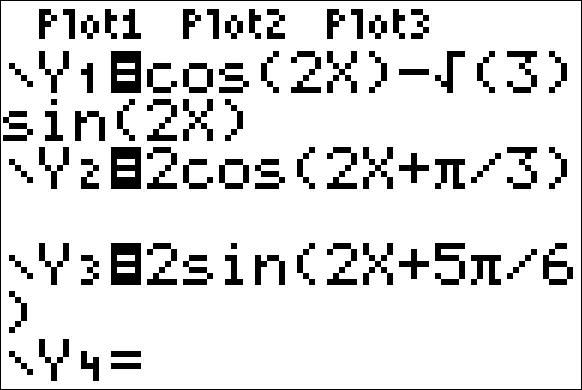
\includegraphics[width=2in]{./IntroTrigGraphics/TrigGraphs01.jpg} &

\hspace{0.75in} 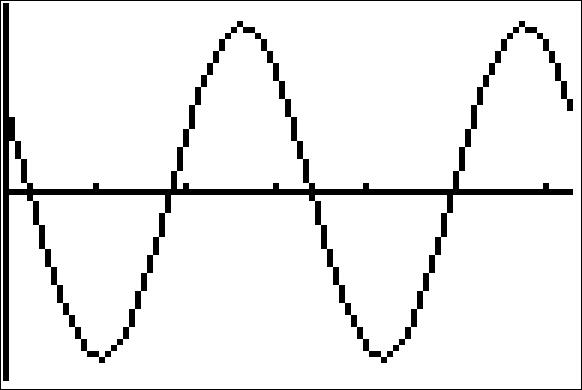
\includegraphics[width=2in]{./IntroTrigGraphics/TrigGraphs02.jpg} \\

\end{tabular}

\end{center}

\qed

\end{enumerate}

\end{ex}

It is important to note that in order for the technique presented in Example \ref{expandedsinusoidex1} to fit a function into one of the forms in Theorem \ref{sinusoidform},  the arguments of the cosine and sine function much match.  That is, while $f(x) = \cos(2x) - \sqrt{3} \sin(2x)$ is a sinusoid, $g(x) =  \cos(2x) - \sqrt{3} \sin(3x)$ is not.\footnote{This graph does, however, exhibit sinusoid-like characteristics!  Check it out!}  It is also worth mentioning that, had we chosen  $A = -2$ instead of $A = 2$ as we worked through Example \ref{expandedsinusoidex1}, our final answers would have \textit{looked} different. The reader is encouraged to rework Example  \ref{expandedsinusoidex1} using $A = -2$ to see what these differences are, and then for a challenging exercise, use identities to show that the formulas are all equivalent.  The general equations to fit a function of the form $f(x) = a \, \cos(\omega x) + b \, \sin(\omega x) + B$ into one of the forms in Theorem \ref{sinusoidform} are explored in Exercise \ref{sinusoidexercise1}.

\subsection{Graphs of the Secant and Cosecant Functions}
\label{secantcosecantgraphsection}

We now turn our attention to graphing $y = \sec(x)$.  Since $\sec(x) = \frac{1}{\cos(x)}$, we can use our table of values for the graph of $y = \cos(x)$ and take reciprocals. We know from Section \ref{circularfunctionsbeyond} that the domain of $F(x) = \sec(x)$ excludes all odd multiples of $\frac{\pi}{2}$, and sure enough, we run into trouble at $x = \frac{\pi}{2}$ and $x = \frac{3\pi}{2}$ since $\cos(x) = 0$ at these values.  Using the notation introduced in Section \ref{RationalGraphs}, we have that as $x \rightarrow \frac{\pi}{2}^{-}$, $\cos(x) \rightarrow 0^{+}$, so $\sec(x) \rightarrow \infty$. (See Section \ref{circularfunctionsbeyond} for a more detailed analysis.) Similarly, we find that  as $x \rightarrow \frac{\pi}{2}^{+}$, $\sec(x) \rightarrow -\infty$;  as $x \rightarrow \frac{3\pi}{2}^{-}$, $\sec(x) \rightarrow -\infty$; and as $x \rightarrow \frac{3\pi}{2}^{+}$, $\sec(x) \rightarrow \infty$.  This means we have a pair of vertical asymptotes to the graph of $y = \sec(x)$, $x = \frac{\pi}{2}$ and $x = \frac{3\pi}{2}$.  Since $\cos(x)$ is periodic with period $2\pi$, it follows that $\sec(x)$ is also.\footnote{Provided $\sec(\alpha)$ and  $\sec(\beta)$ are defined, $\sec(\alpha) = \sec(\beta)$ if and only if $\cos(\alpha) = \cos(\beta)$.  Hence, $\sec(x)$ inherits its period from $\cos(x)$.}  Below we graph a fundamental cycle of $y = \sec(x)$ \index{secant ! graph of} along with a more complete graph obtained by the usual `copying and pasting.'\footnote{In Section \ref{circularfunctionsbeyond}, we argued the range of $F(x) = \sec(x)$ is $(-\infty, -1] \cup [1,\infty)$.  We can now see this graphically.}

\hspace{.25in} \begin{tabular}{m{2.7in}m{3in}}
\setlength{\extrarowheight}{2pt}
\[ \begin{array}{|r||r|r|r|}  

\hline

 x & \cos(x) & \sec(x) & (x,\sec(x)) \\ \hline
0  & 1 & 1 & (0,1) \\ [2pt]   \hline
\frac{\pi}{4}  & \frac{\sqrt{2}}{2} & \sqrt{2} & \left(\frac{\pi}{4}, \sqrt{2} \right) \\ [2pt] \hline 
\frac{\pi}{2}  & 0 & \text{undefined} &  \\ [2pt] \hline 
\frac{3\pi}{4}  & -\frac{\sqrt{2}}{2} & -\sqrt{2} & \left(\frac{3\pi}{4}, -\sqrt{2} \right) \\ [2pt] \hline 
\pi & -1 & -1 &  (\pi, -1) \\ [2pt] \hline 
\frac{5\pi}{4}  & -\frac{\sqrt{2}}{2} & -\sqrt{2} & \left(\frac{5\pi}{4}, -\sqrt{2} \right) \\ [2pt] \hline 
\frac{3\pi}{2}  & 0 & \text{undefined} & \\ [2pt] \hline 
\frac{7\pi}{4}  & \frac{\sqrt{2}}{2} & \sqrt{2} & \left(\frac{7\pi}{4}, \sqrt{2} \right) \\ [2pt] \hline 
2\pi  & 1 &  1& (2\pi, 1) \\  [2pt] \hline
\end{array} \] \setlength{\extrarowheight}{0pt} &

\begin{mfpic}[25]{-1}{7}{-4}{4}
\point[3pt]{(0,1), (0.7854,1.4142),  (2.3562,-1.4142), (3.1416, -1), (3.9270,-1.4142),  (5.4978,1.4142), (6.2832,1)}
\axes
\tlabel[cc](7,-0.25){\scriptsize $x$}
\tlabel[cc](0.25,4){\scriptsize $y$}
\tcaption{The `fundamental cycle' of $y = \sec(x)$.}
\xmarks{0.7854, 1.5708, 2.3562, 3.1416, 3.9270, 4.7124,5.4978,6.2832 }
\ymarks{-3,-2,-1,1,2,3}
\tlpointsep{4pt}
\scriptsize
\axislabels {x}{{$\frac{\pi}{4}$} 0.7854, {$\frac{\pi}{2}$} 1.5708, {$\frac{3\pi}{4}$} 2.3562, {$\pi$} 3.1416, {$\frac{5\pi}{4}$} 3.9270, {$\frac{3\pi}{2}$} 4.7124, {$\frac{7\pi}{4}$} 5.4978, {$2\pi$} 6.2832}
\axislabels {y}{{$-3$} -3,{$-2$} -2,{$-1$} -1, {$1$} 1, {$2$} 2, {$3$} 3}
\normalsize
\dotted \function{0, 6.2832, 0.1}{cos(x)}
\dashed \polyline{(1.5708, -4), (1.5708, 4)}
\dashed \polyline{(4.7124, -4), (4.7124, 4)}
\arrow \function{0, 1.3181, 0.1}{1/cos(x)}
\arrow \reverse \arrow \function{1.8235, 4.460, 0.1}{1/cos(x)}
\arrow \reverse \function{4.9651, 6.28, 0.1}{1/cos(x)}
\end{mfpic} \\

\end{tabular}

\begin{center}

\begin{mfpic}[15]{-13}{13}{-4}{4}
\point[3pt]{(0,1), (3.1416, -1), (6.2832,1)}
\axes
\tlabel[cc](13,-0.25){\scriptsize $x$}
\tlabel[cc](0.25,4){\scriptsize $y$}
\tcaption{The graph of $y = \sec(x)$.}
\tlpointsep{4pt}
\dotted \function{-12.5664, 12.5664, 0.1}{cos(x)}
\dashed \polyline{(1.5708, -4), (1.5708, 4)}
\dashed \polyline{(4.7124, -4), (4.7124, 4)}
\dashed \polyline{(7.8540, -4), (7.8540, 4)}
\dashed \polyline{(10.9956, -4), (10.9956, 4)}
\dashed \polyline{(-1.5708, -4), (-1.5708, 4)}
\dashed \polyline{(-4.7124, -4), (-4.7124, 4)}
\dashed \polyline{(-7.8540, -4), (-7.8540, 4)}
\dashed \polyline{(-10.9956, -4), (-10.9956, 4)}
\arrow \reverse \arrow \function{-1.3181, 1.3181, 0.1}{1/cos(x)}
\arrow \reverse \arrow \function{1.8235, 4.460, 0.1}{1/cos(x)}
\arrow \reverse \arrow \function{4.9651, 7.6013, 0.1}{1/cos(x)}
\arrow \reverse \arrow \function{8.1067, 10.7432, 0.1}{1/cos(x)}
\arrow \reverse \arrow \function{-1.8235, -4.460, -0.1}{1/cos(x)}
\arrow \reverse \arrow \function{-4.9651, -7.6013, -0.1}{1/cos(x)}
\arrow \reverse \arrow \function{-8.1067, -10.7432, -0.1}{1/cos(x)}
\arrow \reverse \function{-11.2483, -12.5664, -0.1}{1/cos(x)}
\arrow \reverse \function{11.2483, 12.5664, 0.1}{1/cos(x)}
\penwd{1.5pt}
\arrow \function{0, 1.3181, 0.1}{1/cos(x)}
\arrow \reverse \arrow \function{1.8235, 4.460, 0.1}{1/cos(x)}
\arrow \reverse \function{4.9651, 6.28, 0.1}{1/cos(x)}
\end{mfpic}

\end{center}

As one would expect, to graph $y = \csc(x)$ we begin with $y = \sin(x)$ and take reciprocals of the corresponding $y$-values.  Here, we encounter issues at $x = 0$, $x = \pi$ and $x = 2\pi$.  Proceeding with the usual analysis, we graph the fundamental cycle of $y = \csc(x)$ below along with the dotted graph of $y=\sin(x)$ for reference.  Since $y = \sin(x)$ and $y = \cos(x)$ are merely phase shifts of each other, so too are $y = \csc(x)$ and $y = \sec(x)$. \index{cosecant ! graph of}

\hspace{.25in} \begin{tabular}{m{2.7in}m{3in}}
\setlength{\extrarowheight}{2pt}
\[ \begin{array}{|r||r|r|r|}  

\hline

 x & \sin(x) & \csc(x) & (x,\csc(x)) \\ \hline
0  & 0 & \text{undefined} &  \\ [2pt]   \hline
\frac{\pi}{4}  & \frac{\sqrt{2}}{2} & \sqrt{2} & \left(\frac{\pi}{4}, \sqrt{2} \right) \\ [2pt] \hline 
\frac{\pi}{2}  & 1 & 1 & \left(\frac{\pi}{2}, 1 \right) \\ [2pt] \hline 
\frac{3\pi}{4}  & \frac{\sqrt{2}}{2} & \sqrt{2} & \left(\frac{3\pi}{4}, \sqrt{2} \right) \\ [2pt] \hline 
\pi & 0 & \text{undefined} &   \\ [2pt] \hline 
\frac{5\pi}{4}  & -\frac{\sqrt{2}}{2} & -\sqrt{2} & \left(\frac{5\pi}{4}, -\sqrt{2} \right) \\ [2pt] \hline 
\frac{3\pi}{2}  & -1 & -1 & \left(\frac{3\pi}{2},-1 \right)\\ [2pt] \hline 
\frac{7\pi}{4}  & -\frac{\sqrt{2}}{2} & -\sqrt{2} & \left(\frac{7\pi}{4}, -\sqrt{2} \right) \\ [2pt] \hline 
2\pi  & 0 & \text{undefined} &  \\  [2pt] \hline
\end{array} \] \setlength{\extrarowheight}{0pt} &

\begin{mfpic}[25]{-1}{7}{-4}{4.25}
\point[3pt]{ (0.7854,1.4142), (1.5708, 1) ,(2.3562,1.4142), (4.7124, -1), (3.9270,-1.4142),  (5.4978,-1.4142)}
\axes
\tlabel[cc](7,-0.25){\scriptsize $x$}
\tlabel[cc](0.25,4.25){\scriptsize $y$}
\tcaption{The `fundamental cycle' of $y = \csc(x)$.}
\xmarks{0.7854, 1.5708, 2.3562, 3.1416, 3.9270, 4.7124,5.4978,6.2832 }
\ymarks{-3,-2,-1,1,2,3}
\tlpointsep{4pt}
\scriptsize 
\axislabels {x}{{$\frac{\pi}{4}$} 0.7854, {$\frac{\pi}{2}$} 1.5708, {$\frac{3\pi}{4}$} 2.3562, {$\pi$} 3.1416, {$\frac{5\pi}{4}$} 3.9270, {$\frac{3\pi}{2}$} 4.7124, {$\frac{7\pi}{4}$} 5.4978, {$2\pi$} 6.2832}
\axislabels {y}{{$-3$} -3,{$-2$} -2,{$-1$} -1, {$1$} 1, {$2$} 2, {$3$} 3}
\normalsize
\dotted \function{0, 6.2832, 0.1}{sin(x)}
\dashed \polyline{(3.1416, -4), (3.1416, 4)}
\dashed \polyline{(6.2832, -4), (6.2832, 4)}
\arrow \reverse \arrow \function{0.2527, 2.889, 0.1}{1/sin(x)}
\arrow \reverse \arrow \function{3.3943, 6.0306, 0.1}{1/sin(x)}
\end{mfpic} \\

\end{tabular}

Once again, our domain and range work in Section \ref{circularfunctionsbeyond} is verified geometrically in the graph of $y = G(x) = \csc(x)$.


\begin{center}

\begin{mfpic}[15]{-13}{13}{-4}{4.25}
\point[3pt]{ (1.5708, 1), (4.7124, -1)}
\axes
\tlabel[cc](13,-0.25){\scriptsize $x$}
\tlabel[cc](0.25,4.25){\scriptsize $y$}
\tcaption{The graph of $y = \csc(x)$.}
\tlpointsep{4pt}
\dotted \function{-12.5664, 12.5664, 0.1}{sin(x)}
\dashed \polyline{(3.1416, -4), (3.1416, 4)}
\dashed \polyline{(6.2832, -4), (6.2832, 4)}
\dashed \polyline{(-3.1416, -4), (-3.1416, 4)}
\dashed \polyline{(-6.2832, -4), (-6.2832, 4)}
\dashed \polyline{(9.4248, -4), (9.4248, 4)}
\dashed \polyline{(12.5664, -4), (12.5664, 4)}
\dashed \polyline{(-9.4248, -4), (-9.4248, 4)}
\dashed \polyline{(-12.5664, -4), (-12.5664, 4)}
\arrow \reverse \arrow \function{0.2527, 2.889, 0.1}{1/sin(x)}
\arrow \reverse \arrow \function{3.3943, 6.0306, 0.1}{1/sin(x)}
\arrow \reverse \arrow \function{-0.2527, -2.889, -0.1}{1/sin(x)}
\arrow \reverse \arrow \function{-3.3943, -6.0306, -0.1}{1/sin(x)}
\arrow \reverse \arrow \function{6.5359, 9.1723, 0.1}{1/sin(x)}
\arrow \reverse \arrow \function{-6.5359, -9.1723, -0.1}{1/sin(x)}
\arrow \reverse \arrow \function{9.6775, 12.3138, 0.1}{1/sin(x)}
\arrow \reverse \arrow \function{-9.6775, -12.3138, -0.1}{1/sin(x)}
\penwd{1.5pt}
\arrow \reverse \arrow \function{0.2527, 2.889, 0.1}{1/sin(x)}
\arrow \reverse \arrow \function{3.3943, 6.0306, 0.1}{1/sin(x)}
\end{mfpic}

\end{center}

Note that, on the intervals between the vertical asymptotes, both $F(x) = \sec(x)$ and $G(x) = \csc(x)$ are continuous and smooth.  In other words, they are continuous and smooth \textit{on their domains}.\footnote{Just like the rational functions in Chapter \ref{Rationals} are continuous and smooth on their domains because polynomials are continuous and smooth everywhere, the secant and cosecant functions are continuous and smooth on their domains since the cosine and sine functions are continuous and smooth everywhere.}  The following theorem summarizes the properties of the secant and cosecant functions.  Note that all of these properties are direct results of them being reciprocals of the cosine and sine functions, respectively.

\smallskip

\colorbox{ResultColor}{\bbm

\begin{thm} \label{secantcosecantfunctionprops}  \textbf{Properties of the Secant and Cosecant Functions} \index{secant ! properties of} \index{cosecant ! properties of}

\begin{itemize}

\item  The function $F(x) = \sec(x)$

\begin{itemize}


\item has domain $\left\{ x : x \neq \frac{\pi}{2} + \pi k, \, \,  \text{$k$ is an integer} \right\} = \displaystyle{\bigcup_{k=-\infty}^{\infty} \left(\frac{(2k+1) \pi}{2}, \frac{(2k+3) \pi}{2}\right)}$

\item has range $\{ y : |y| \geq 1 \} = (-\infty, -1] \cup [1, \infty)$

\item  is continuous and smooth on its domain

\item is even

\item has period $2\pi$

\end{itemize}

\item  The function $G(x) = \csc(x)$

\begin{itemize}

\item has domain $\left\{ x : x \neq \pi  k, \, \,  \text{$k$ is an integer} \right\} = \displaystyle{\bigcup_{k=-\infty}^{\infty}\left(k\pi, (k+1) \pi \right)}$

\item has range $\{ y : |y| \geq 1 \} = (-\infty, -1] \cup [1, \infty)$

\item  is continuous and smooth on its domain

\item is odd

\item has period $2\pi$

\end{itemize}

\end{itemize}

\end{thm}

\ebm}

\medskip

In the next example, we discuss graphing more general secant and cosecant curves.

\begin{ex}  \label{seccscgraphex} Graph one cycle of the following functions.  State the period of each.

\begin{multicols}{2}

\begin{enumerate}

\item  $f(x) = 1 - 2 \sec(2x)$

\item  $g(x) = \dfrac{\csc(\pi - \pi x) - 5}{3}$

\end{enumerate}

\end{multicols}

{\bf Solution.}  

\begin{enumerate}

\item  To graph $y = 1 - 2 \sec(2x)$, we follow the same procedure as in Example \ref{cosinesinegraphex1}.  First, we set the argument of secant, $2x$, equal to the `quarter marks' $0$, $\frac{\pi}{2}$, $\pi$, $\frac{3\pi}{2}$ and $2\pi$ and solve for $x$.

\setlength{\extrarowheight}{2pt}
\[ \begin{array}{|r|r|r|}  

\hline

 a & 2x = a & x \\ [2pt] \hline
0  & 2x = 0 & 0 \\ [2pt]   \hline

\frac{\pi}{2}  & 2x = \frac{\pi}{2} & \frac{\pi}{4} \\ [2pt] \hline 

\pi &  2x = \pi & \frac{\pi}{2} \\ [2pt] \hline 

\frac{3\pi}{2}  &  2x = \frac{3\pi}{2} & \frac{3\pi}{4} \\ [2pt] \hline 

2\pi  & 2x = 2\pi & \pi \\  [2pt] \hline
\end{array} \]
\setlength{\extrarowheight}{0pt}

Next, we substitute these $x$ values into $f(x)$.  If $f(x)$ exists, we have a point on the graph;  otherwise, we have found a vertical asymptote.  In addition to these points and asymptotes, we have graphed the associated cosine curve -- in this case $y = 1 - 2 \cos(2x)$ -- dotted in the picture below.  Since one cycle is graphed over the interval $[0,\pi]$, the period is $\pi - 0 = \pi$.
 

\hspace{.25in} \begin{tabular}{m{2.7in}m{3in}}
\setlength{\extrarowheight}{2pt}
\[ \begin{array}{|r||r|r|}  

\hline

 x & f(x) & (x,f(x))  \\ \hline
0  & - 1 & (0,-1)  \\ [2pt]   \hline
\frac{\pi}{4}  & \text{undefined} &  \\ [2pt] \hline 
\frac{\pi}{2}  & 3 & \left(\frac{\pi}{2}, 3 \right)  \\ [2pt] \hline 
\frac{3\pi}{4}  & \text{undefined} &  \\ [2pt] \hline 
\pi & -1 &   (\pi, -1) \\ [2pt] \hline 
\end{array} \] \setlength{\extrarowheight}{0pt} &

\begin{mfpic}[27][9]{-1}{4}{-7}{9}
\point[3pt]{(0,-1), (1.5708,3),  (3.1416, -1)}
\axes
\tlabel[cc](4,-0.3){\scriptsize $x$}
\tlabel[cc](0.25,9){\scriptsize $y$}
\tcaption{One cycle of $y = 1-2\sec(2x)$.}
\xmarks{0.7854, 1.5708, 2.3562, 3.1416}
\ymarks{-1,1,2,3}
\tlpointsep{4pt}
\scriptsize 
\axislabels {x}{{$\frac{\pi}{4}$} 0.7854, {$\frac{\pi}{2}$} 1.5708, {$\frac{3\pi}{4}$} 2.3562, {$\pi$} 3.1416}
\normalsize
\axislabels {y}{{\scriptsize $-1$} -1, {\scriptsize $1$} 1, {\scriptsize $2$} 2, {\scriptsize $3$} 3}
\dotted \function{0, 3.1416, 0.1}{1 - 2*cos(2*x)}
\dashed \polyline{(0.7854, -7), (0.7854, 9)}
\dashed \polyline{(2.3562, -7), (2.3562, 9)}
\arrow \function{0, 0.6590, 0.1}{1-2/cos(2*x)}
\arrow \reverse \arrow \function{0.9118, 2.230, 0.1}{1-2/cos(2*x)}
\arrow \reverse \function{2.4826, 3.14, 0.1}{1-2/cos(2*x)}
\end{mfpic} \\

\end{tabular}



\item  Proceeding as before, we set the argument of cosecant in $g(x) = \frac{\csc(\pi - \pi x) - 5}{3}$ equal to the quarter marks and solve for $x$.

\setlength{\extrarowheight}{2pt}
\[ \begin{array}{|r|r|r|}  

\hline

 a & \pi - \pi x = a & x \\ [2pt] \hline
0  & \pi - \pi x = 0 & 1 \\ [2pt]   \hline

\frac{\pi}{2}  & \pi - \pi x = \frac{\pi}{2} & \frac{1}{2} \\ [2pt] \hline 

\pi &  \pi - \pi x = \pi & 0 \\ [2pt] \hline 

\frac{3\pi}{2}  &  \pi - \pi x = \frac{3\pi}{2} & -\frac{1}{2} \\ [2pt] \hline 

2\pi  & \pi - \pi x = 2\pi & -1 \\  [2pt] \hline
\end{array} \]
\setlength{\extrarowheight}{0pt}

Substituting these $x$-values into $g(x)$, we generate the graph below and find the period to be $1 - (-1) = 2$.   The associated sine curve, $y = \frac{\sin(\pi - \pi x) - 5}{3}$, is dotted in as a reference.  

\hspace{.25in} \begin{tabular}{m{2.7in}m{3in}}
\setlength{\extrarowheight}{2pt}
\[ \begin{array}{|r||r|r|}  

\hline

 x & g(x) & (x,g(x))  \\ \hline
1  & \text{undefined} &   \\ [2pt]   \hline
\frac{1}{2}  & -\frac{4}{3} &  \left(\frac{1}{2}, -\frac{4}{3} \right)  \\ [2pt] \hline 
0 & \text{undefined} &   \\ [2pt] \hline 
-\frac{1}{2} & -2 & \left(-\frac{1}{2}, -2\right)  \\ [2pt] \hline 
-1 & \text{undefined} &    \\ [2pt] \hline 
\end{array} \] \setlength{\extrarowheight}{0pt} &

\begin{mfpic}[30]{-2}{2}{-3}{0.5}
\point[3pt]{(0.5,-1.3333),  (-0.5, -2)}
\axes
\tlabel[cc](2,-0.3){\scriptsize $x$}
\tlabel[cc](0.25,0.5){\scriptsize $y$}
\tcaption{One cycle of $y = \frac{\csc(\pi - \pi x) - 5}{3}$.}
\xmarks{-1, -0.5, 0.5, 1}
\ymarks{-2,-1}
\tlpointsep{4pt}
\axislabels {x}{{\scriptsize $-1 \hspace{7pt}$} -1, {\scriptsize $-\frac{1}{2} \hspace{7pt}$} -0.5, {\scriptsize $\frac{1}{2}$} 0.5, {\scriptsize $1$} 1}
\axislabels {y}{{\scriptsize $-2$} -2, {\scriptsize $-1$} -1}
\dotted \function{-1, 1, 0.1}{(sin(3.14159 - 3.14159*x)-5)/3}
\dashed \polyline{(-1, -3), (-1, -0.5)}
\dashed \polyline{(1, -3), (1,-0.5)}
\arrow \reverse \arrow \function{0.9196, 0.08040, -0.1}{((1/sin(3.14159 - 3.14159*x))-5)/3}
\arrow \reverse \arrow \function{-0.08043, -0.9196, 0.1}{((1/sin(3.14159 - 3.14159*x))-5)/3}
\end{mfpic} \\

\end{tabular}

\vspace{-0.2in}  \qed

\end{enumerate}

\end{ex}

Before moving on, we note that it is possible to speak of the period, phase shift and vertical shift of secant and cosecant graphs and use even/odd identities to put them in a form similar to the sinusoid forms mentioned in Theorem \ref{sinusoidform}.  Since these quantities match those of the corresponding cosine and sine curves, we do not spell this out explicitly.  Finally, since the ranges of secant and cosecant are unbounded, there is no amplitude associated with these curves.

\subsection{Graphs of the Tangent and Cotangent Functions}

Finally, we turn our attention to the graphs of the tangent and cotangent functions.  When constructing a table of values for the tangent function, we see that $J(x) = \tan(x)$ is undefined at $x  = \frac{\pi}{2}$ and $x = \frac{3\pi}{2}$, in accordance with our findings in Section \ref{circularfunctionsbeyond}.  As $x \rightarrow \frac{\pi}{2}^{-}$, $\sin(x) \rightarrow 1^{-}$ and $\cos(x) \rightarrow 0^{+}$, so that $\tan(x)  = \frac{\sin(x)}{\cos(x)}\rightarrow \infty$ producing a vertical asymptote at $x = \frac{\pi}{2}$.  Using a similar analysis, we get that as $x \rightarrow \frac{\pi}{2}^{+}$, $\tan(x) \rightarrow -\infty$; as $x \rightarrow \frac{3\pi}{2}^{-}$, $\tan(x) \rightarrow \infty$; and as $x \rightarrow \frac{3\pi}{2}^{+}$, $\tan(x) \rightarrow -\infty$.  Plotting this information and performing the usual `copy and paste' produces: \index{tangent ! graph of}


\hspace{.5in} \begin{tabular}{m{2.7in}m{3in}}
\setlength{\extrarowheight}{2pt}
\[ \begin{array}{|r||r|r|}  

\hline

 x & \tan(x) & (x,\tan(x)) \\ \hline
0  & 0 & (0, 0) \\ [2pt]   \hline
\frac{\pi}{4}  & 1 & \left(\frac{\pi}{4},1 \right) \\ [2pt] \hline 
\frac{\pi}{2}  & \text{undefined} &  \\ [2pt] \hline 
\frac{3\pi}{4}  & -1 & \left(\frac{3\pi}{4}, -1\right) \\ [2pt] \hline 
\pi & 0 & (\pi, 0) \\ [2pt] \hline 
\frac{5\pi}{4}  & 1 & \left(\frac{5\pi}{4}, 1 \right) \\ [2pt] \hline 
\frac{3\pi}{2}  & \text{undefined} &  \\ [2pt] \hline 
\frac{7\pi}{4}  & -1 & \left(\frac{7\pi}{4}, -1 \right) \\ [2pt] \hline 
2\pi  & 0 & (2\pi, 0) \\  [2pt] \hline
\end{array} \] \setlength{\extrarowheight}{0pt} &

\begin{mfpic}[25]{-1}{7}{-4}{4}
\point[3pt]{(0,0), (0.7854,1), (2.3562,-1), (3.1416, 0), (3.9270,1),  (5.4978,-1), (6.2832,0)}
\dashed \polyline{(1.5708,-4), (1.5708,4)}
\dashed \polyline{(4.7124,-4), (4.7124,4)}
\axes
\tlabel[cc](7,-0.25){\scriptsize $x$}
\tlabel[cc](0.25,4){\scriptsize $y$}
\tcaption{The graph of $y = \tan(x)$ over $[0,2\pi]$.}
\xmarks{0.7854, 1.5708, 2.3562, 3.1416, 3.9270, 4.7124,5.4978,6.2832 }
\ymarks{-1,1}
\tlpointsep{4pt}
\scriptsize
\axislabels {x}{{$\frac{\pi}{4}$} 0.7854, {$\frac{\pi}{2}$} 1.5708, {$\frac{3\pi}{4}$} 2.3562, {$\pi$} 3.1416, {$\frac{5\pi}{4}$} 3.9270, {$\frac{3\pi}{2}$} 4.7124, {$\frac{7\pi}{4}$} 5.4978, {$2\pi$} 6.2832}
\axislabels {y}{{$-1$} -1, {$1$} 1}
\normalsize
\arrow \function{0, 1.3258, 0.1}{tan(x)}
\arrow \reverse \arrow \function{1.8158, 4.4674, 0.1}{tan(x)}
\arrow \reverse \function{4.9574, 6.2832,0.1}{tan(x)}
\end{mfpic} \\

\end{tabular}



\begin{center}

\begin{mfpic}[15]{-13}{13}{-4}{4}
\point[3pt]{(-0.7854,-1), (0,0), (0.7854,1)}
\axes
\tlabel[cc](13,-0.25){\scriptsize $x$}
\tlabel[cc](0.25,4){\scriptsize $y$}
\tcaption{The graph of $y = \tan(x)$.}
\tlpointsep{4pt}
\dashed \polyline{(1.5708, -4), (1.5708, 4)}
\dashed \polyline{(4.7124, -4), (4.7124, 4)}
\dashed \polyline{(7.8540, -4), (7.8540, 4)}
\dashed \polyline{(10.9956, -4), (10.9956, 4)}
\dashed \polyline{(-1.5708, -4), (-1.5708, 4)}
\dashed \polyline{(-4.7124, -4), (-4.7124, 4)}
\dashed \polyline{(-7.8540, -4), (-7.8540, 4)}
\dashed \polyline{(-10.9956, -4), (-10.9956, 4)}
\arrow \reverse \arrow \function{-1.3181, 1.3181, 0.1}{tan(x)}
\arrow \reverse \arrow \function{1.8235, 4.460, 0.1}{tan(x)}
\arrow \reverse \arrow \function{4.9651, 7.6013, 0.1}{tan(x)}
\arrow \reverse \arrow \function{8.1067, 10.7432, 0.1}{tan(x)}
\arrow \reverse \arrow \function{-1.8235, -4.460, -0.1}{tan(x)}
\arrow \reverse \arrow \function{-4.9651, -7.6013, -0.1}{tan(x)}
\arrow \reverse \arrow \function{-8.1067, -10.7432, -0.1}{tan(x)}
\arrow \reverse \function{-11.2483, -12.5664, -0.1}{tan(x)}
\arrow \reverse \function{11.2483, 12.5664, 0.1}{tan(x)}
\penwd{1.5pt}
\arrow \reverse \arrow \function{-1.3181, 1.3181, 0.1}{tan(x)}
\end{mfpic}

\end{center}

From the graph, it appears as if the tangent function is periodic with period $\pi$.  To prove that this is the case, we appeal to the sum formula for tangents.  We have: \[ \tan(x+\pi) = \dfrac{\tan(x) + \tan(\pi)}{1 - \tan(x) \tan(\pi)} = \dfrac{\tan(x) + 0}{1 - (\tan(x) )(0)} = \tan(x),\]

which tells us the period of $\tan(x)$ is at most $\pi$.  To show that it is exactly $\pi$, suppose $p$ is a positive real number so that $\tan(x+p) = \tan(x)$ for all real numbers $x$.  For $x=0$, we have $\tan(p) = \tan(0+p) = \tan(0) = 0$, which means $p$ is a multiple of $\pi$.  The smallest positive multiple of $\pi$ is $\pi$ itself, so we have established the result.   We take as our fundamental cycle for $y=\tan(x)$ the interval $\left(-\frac{\pi}{2}, \frac{\pi}{2}\right)$, and use as our `quarter marks' $x = -\frac{\pi}{2}$, $-\frac{\pi}{4}$, $0$, $\frac{\pi}{4}$ and $\frac{\pi}{2}$. From the graph, we see confirmation of our domain and range work  in Section \ref{circularfunctionsbeyond}. 

\smallskip

It should be no surprise that $K(x) = \cot(x)$ behaves similarly to $J(x) = \tan(x)$. Plotting $\cot(x)$ over the interval $[0,2\pi]$ results in the graph below. \index{cotangent ! graph of}

\hspace{.5in} \begin{tabular}{m{2.7in}m{3in}}
\setlength{\extrarowheight}{2pt}
\[ \begin{array}{|r||r|r|}  

\hline

 x & \cot(x) & (x,\cot(x)) \\ \hline
0  & \text{undefined} &  \\ [2pt]   \hline
\frac{\pi}{4}  & 1 & \left(\frac{\pi}{4},1 \right) \\ [2pt] \hline 
\frac{\pi}{2}  & 0 & \left(\frac{\pi}{2},0 \right)  \\ [2pt] \hline 
\frac{3\pi}{4}  & -1 & \left(\frac{3\pi}{4}, -1\right) \\ [2pt] \hline 
\pi & \text{undefined} &  \\ [2pt] \hline 
\frac{5\pi}{4}  & 1 & \left(\frac{5\pi}{4}, 1 \right) \\ [2pt] \hline 
\frac{3\pi}{2}  & 0 & \left(\frac{3\pi}{2}, 0 \right) \\ [2pt] \hline 
\frac{7\pi}{4}  & -1 & \left(\frac{7\pi}{4}, -1 \right) \\ [2pt] \hline 
2\pi  & \text{undefined} &  \\  [2pt] \hline
\end{array} \] \setlength{\extrarowheight}{0pt} &

\begin{mfpic}[25]{-1}{7}{-4}{4.25}
\point[3pt]{ (0.7854,1), (1.5708,0), (2.3562,-1), (3.9270,1), (4.7124,0), (5.4978,-1)}
\dashed \polyline{(3.1416,-4), (3.1416,4)}
\dashed \polyline{(6.2832,-4), (6.2832,4)}
\axes
\tlabel[cc](7,-0.25){\scriptsize $x$}
\tlabel[cc](0.25,4.25){\scriptsize $y$}
\tcaption{The graph of $y = \cot(x)$ over $[0,2\pi]$.}
\xmarks{0.7854, 1.5708, 2.3562, 3.1416, 3.9270, 4.7124,5.4978,6.2832 }
\ymarks{-1,1}
\tlpointsep{4pt}
\scriptsize
\axislabels {x}{{$\frac{\pi}{4}$} 0.7854, {$\frac{\pi}{2}$} 1.5708, {$\frac{3\pi}{4}$} 2.3562, {$\pi$} 3.1416, {$\frac{5\pi}{4}$} 3.9270, {$\frac{3\pi}{2}$} 4.7124, {$\frac{7\pi}{4}$} 5.4978, {$2\pi$} 6.2832}
\axislabels {y}{{$-1$} -1, {$1$} 1}
\normalsize
\arrow \reverse \arrow \function{0.2450, 2.8966, 0.1}{cot(x)}
\arrow \reverse \arrow \function{3.3865, 6.0382,0.1}{cot(x)}
\end{mfpic} \\

\end{tabular}

From these data, it clearly appears as if the period of $\cot(x)$ is $\pi$, and we leave it to the reader to prove this.\footnote{Certainly, mimicking the proof that the period of $\tan(x)$ is an option;  for another approach, consider transforming $\tan(x)$ to $\cot(x)$ using identities.}  We take as one fundamental cycle the interval $(0,\pi)$ with quarter marks:  $x= 0$, $\frac{\pi}{4}$, $\frac{\pi}{2}$, $\frac{3\pi}{4}$ and $\pi$.  A more complete graph of $y=\cot(x)$ is below, along with the fundamental cycle highlighted as usual.  Once again, we see the domain and range of $K(x) = \cot(x)$ as read from the graph matches with what we found analytically in Section \ref{circularfunctionsbeyond}.     

\begin{center}

\begin{mfpic}[15]{-13}{13}{-4}{4.25}
\point[3pt]{ (0.7854,1), (1.5708,0), (2.3562,-1)}
\axes
\tlabel[cc](13,-0.25){\scriptsize $x$}
\tlabel[cc](0.25,4.25){\scriptsize $y$}
\tcaption{The graph of $y = \cot(x)$.}
\tlpointsep{4pt}
\dashed \polyline{(3.1416, -4), (3.1416, 4)}
\dashed \polyline{(6.2832, -4), (6.2832, 4)}
\dashed \polyline{(-3.1416, -4), (-3.1416, 4)}
\dashed \polyline{(-6.2832, -4), (-6.2832, 4)}
\dashed \polyline{(9.4248, -4), (9.4248, 4)}
\dashed \polyline{(12.5664, -4), (12.5664, 4)}
\dashed \polyline{(-9.4248, -4), (-9.4248, 4)}
\dashed \polyline{(-12.5664, -4), (-12.5664, 4)}
\arrow \reverse \arrow \function{0.2527, 2.889, 0.1}{cot(x)}
\arrow \reverse \arrow \function{3.3943, 6.0306, 0.1}{cot(x)}
\arrow \reverse \arrow \function{-0.2527, -2.889, -0.1}{cot(x)}
\arrow \reverse \arrow \function{-3.3943, -6.0306, -0.1}{cot(x)}
\arrow \reverse \arrow \function{6.5359, 9.1723, 0.1}{cot(x)}
\arrow \reverse \arrow \function{-6.5359, -9.1723, -0.1}{cot(x)}
\arrow \reverse \arrow \function{9.6775, 12.3138, 0.1}{cot(x)}
\arrow \reverse \arrow \function{-9.6775, -12.3138, -0.1}{cot(x)}
\penwd{1.5pt}
\arrow \reverse \arrow \function{0.2527, 2.889, 0.1}{cot(x)}
\end{mfpic}

\end{center}

The properties of the tangent and cotangent functions are summarized below. As with Theorem \ref{secantcosecantfunctionprops}, each of the results below can be traced back to properties of the cosine and sine functions and the definition of the tangent and cotangent functions as quotients thereof. 

\smallskip

\colorbox{ResultColor}{\bbm

\begin{thm} \label{tangentcotangentfunctionprops}  \textbf{Properties of the Tangent and Cotangent Functions} \index{tangent ! properties of} \index{cotangent ! properties of}

\begin{itemize}

\item  The function $J(x) = \tan(x)$

\begin{itemize}


\item has domain $\left\{ x : x \neq \frac{\pi}{2} + \pi k, \, \,  \text{$k$ is an integer} \right\} = \displaystyle{\bigcup_{k=-\infty}^{\infty} \left(\frac{(2k+1) \pi}{2}, \frac{(2k+3) \pi}{2}\right)}$

\item has range $(-\infty, \infty)$

\item is continuous and smooth on its domain

\item is odd

\item has period $\pi$

\end{itemize}

\item  The function $K(x) = \cot(x)$

\begin{itemize}

\item has domain $\left\{ x : x \neq \pi  k, \, \,  \text{$k$ is an integer} \right\} = \displaystyle{\bigcup_{k=-\infty}^{\infty}\left(k\pi, (k+1) \pi \right)}$

\item has range $(-\infty, \infty)$

\item is continuous and smooth on its domain

\item is odd

\item has period $\pi$

\end{itemize}

\end{itemize}

\end{thm}

\ebm}

\pagebreak

\begin{ex} \label{tancotgraphex} Graph one cycle of the following functions.  Find the period.

\begin{multicols}{2}

\begin{enumerate}

\item  $f(x) = 1 - \tan\left(\frac{x}{2}\right)$.

\item  $g(x) = 2\cot\left(\frac{\pi}{2} x + \pi\right) + 1$.

\end{enumerate}

\end{multicols}


{\bf Solution.}  

\begin{enumerate}

\item We proceed as we have in all of the previous graphing examples by setting the argument of tangent in $f(x) = 1 - \tan\left(\frac{x}{2}\right)$, namely $\frac{x}{2}$, equal to each of the `quarter marks' $-\frac{\pi}{2}$, $-\frac{\pi}{4}$, $0$, $\frac{\pi}{4}$ and $\frac{\pi}{2}$, and solving for $x$.

\setlength{\extrarowheight}{2pt}
\[ \begin{array}{|r|r|r|}  

\hline

 a & \frac{x}{2} = a & x \\ [2pt] \hline
-\frac{\pi}{2}  & \frac{x}{2} = -\frac{\pi}{2} & -\pi \\ [2pt]   \hline

-\frac{\pi}{4}  &\frac{x}{2} = -\frac{\pi}{4} & - \frac{\pi}{2} \\ [2pt] \hline 

0 &  \frac{x}{2} = 0 & 0 \\ [2pt] \hline 

\frac{\pi}{4}  &  \frac{x}{2} = \frac{\pi}{4} & \frac{\pi}{2} \\ [2pt] \hline 

\frac{\pi}{2}  & \frac{x}{2} = \frac{\pi}{2}  & \pi \\  [2pt] \hline
\end{array} \]
\setlength{\extrarowheight}{0pt}

Substituting these $x$-values into $f(x)$, we find points on the graph and the vertical asymptotes.

\hspace{.25in} \begin{tabular}{m{2.7in}m{3in}}
\setlength{\extrarowheight}{2pt}
\[ \begin{array}{|r||r|r|}  

\hline

 x & f(x) & (x,f(x))  \\ \hline
-\pi  & \text{undefined} &   \\ [2pt]   \hline
-\frac{\pi}{2}  &  2 &  \left(-\frac{\pi}{2}, 2 \right) \\ [2pt] \hline 
0 & 1 &  (0,1)  \\ [2pt] \hline 
\frac{\pi}{2}  & 0 &  \left(\frac{\pi}{2}, 0 \right) \\ [2pt] \hline 
\pi & \text{undefined} &  \\ [2pt] \hline 
\end{array} \] \setlength{\extrarowheight}{0pt} &

\begin{mfpic}[20]{-4}{4}{-3}{5}
\point[3pt]{(-1.5708,2),(0,1), (1.5708,0)}
\axes
\tlabel[cc](4,-0.3){\scriptsize $x$}
\tlabel[cc](0.25,5){\scriptsize $y$}
\tcaption{One cycle of $y = 1 - \tan\left(\frac{x}{2}\right)$.}
\xmarks{ -3.1416, -1.5708, 1.5708, 3.1416}
\ymarks{-2,-1,1,2}
\tlpointsep{4pt}
\scriptsize
\axislabels {x}{{$-\pi \hspace{7pt}$} -3.1416,{$-\frac{\pi}{2} \hspace{7pt}$} -1.5708, {$\frac{\pi}{2}$} 1.5708,, {$\pi$} 3.1416}
\normalsize
\axislabels {y}{{\scriptsize $-2$} -2,{\scriptsize $-1$} -1, {\scriptsize $1$} 1, {\scriptsize $2$} 2}
\dashed \polyline{(-3.1416, -3), (-3.1416, 5)}
\dashed \polyline{(3.1416, -3), (3.1416, 5)}
\arrow \reverse \arrow \function{-2.6516, 2.6516, 0.1}{1-tan(0.5*x)}
\end{mfpic} \\

\end{tabular}

We see that the period is $\pi - (-\pi) = 2\pi$.

\item  The `quarter marks' for the fundamental cycle of the cotangent curve are $0$, $\frac{\pi}{4}$, $\frac{\pi}{2}$, $\frac{3\pi}{4}$ and $\pi$.  To graph $g(x) = 2\cot\left(\frac{\pi}{2} x + \pi\right) + 1$, we begin by setting $\frac{\pi}{2} x + \pi$ equal to each quarter mark and solving for $x$.


\setlength{\extrarowheight}{2pt}
\[ \begin{array}{|r|r|r|}  

\hline

 a & \frac{\pi}{2} x + \pi = a & x \\ [2pt] \hline
0  & \frac{\pi}{2} x + \pi = 0 &  -2 \\ [2pt]   \hline

\frac{\pi}{4}  &  \frac{\pi}{2} x + \pi  = \frac{\pi}{4} & -\frac{3}{2} \\ [2pt] \hline 

\frac{\pi}{2}  &  \frac{\pi}{2} x + \pi = \frac{\pi}{2} & -1 \\ [2pt] \hline 

\frac{3\pi}{4}  &  \frac{\pi}{2} x + \pi =\frac{3\pi}{4} & -\frac{1}{2} \\ [2pt] \hline 

\pi  & \frac{\pi}{2} x + \pi = \pi   &  0 \\  [2pt] \hline
\end{array} \]
\setlength{\extrarowheight}{0pt}

We now use these $x$-values to generate our graph.

\hspace{.25in} \begin{tabular}{m{2.7in}m{3in}}
\setlength{\extrarowheight}{2pt}
\[ \begin{array}{|r||r|r|}  

\hline

 x & g(x) & (x,g(x))  \\ \hline
-2  & \text{undefined} &   \\ [2pt]   \hline
-\frac{3}{2}  &  3 &  \left(-\frac{3}{2}, 3 \right) \\ [2pt] \hline 
-1 & 1 &  (-1,1)  \\ [2pt] \hline 
-\frac{1}{2}  & -1 &  \left(-\frac{1}{2}, -1 \right) \\ [2pt] \hline 
0 & \text{undefined} &  \\ [2pt] \hline 
\end{array} \] \setlength{\extrarowheight}{0pt} &

\begin{mfpic}[30][20]{-3}{1}{-2}{4}
\point[3pt]{(-1.5,3),(-1,1), (-0.5,-1)}
\axes
\tlabel[cc](1,-0.3){\scriptsize $x$}
\tlabel[cc](0.25,4){\scriptsize $y$}
\tcaption{\scriptsize One cycle of $y = 2\cot\left(\frac{\pi}{2} x + \pi\right) + 1$.}
\xmarks{ -2, -1}
\ymarks{-1,1,2,3}
\tlpointsep{4pt}
\axislabels {x}{{\scriptsize $-2 \hspace{7pt}$} -2,{\scriptsize $-1 \hspace{7pt}$} -1}
\axislabels {y}{{\scriptsize $-1$} -1,{\scriptsize $1$} 1, {\scriptsize $2$} 2, {\scriptsize $3$} 3}
\dashed \polyline{(-2, -2), (-2, 4)}
\arrow \reverse \arrow \function{-1.62566, -0.3743, 0.1}{1+2*cot((1.5708*x)+ 3.1416)}
\end{mfpic} \\

\end{tabular}

We find the period to be $0 - (-2) = 2$. \qed

\end{enumerate}
\end{ex}

As with the secant and cosecant functions, it is possible to extend the notion of period, phase shift and vertical shift to the tangent and cotangent functions as we did for the cosine and sine functions in Theorem \ref{sinusoidform}.  Since the number of classical applications involving sinusoids far outnumber those involving tangent and cotangent functions, we omit this.  The ambitious reader is invited to formulate such a theorem, however.

\newpage

\subsection{Exercises}

In Exercises \ref{sinecosinegraphfirst} - \ref{sinecosinegraphlast}, graph one cycle of the given function.  State the period, amplitude, phase shift and vertical shift of the function.

\begin{multicols}{3}

\begin{enumerate}

\item $y = 3\sin(x)$ \label{sinecosinegraphfirst}
\item $y = \sin(3x)$
\item $y = -2\cos(x)$

\setcounter{HW}{\value{enumi}}

\end{enumerate}

\end{multicols}

\begin{multicols}{3}

\begin{enumerate}

\setcounter{enumi}{\value{HW}}

\item $y = \cos \left( x - \dfrac{\pi}{2} \right)$
\item $y = -\sin \left( x + \dfrac{\pi}{3} \right)$
\item $y = \sin(2x - \pi)$ \vphantom{$\left( \dfrac{\pi}{2} \right)$}

\setcounter{HW}{\value{enumi}}

\end{enumerate}

\end{multicols}

\begin{multicols}{3}

\begin{enumerate}

\setcounter{enumi}{\value{HW}}

\item $y = -\dfrac{1}{3}\cos \left( \dfrac{1}{2}x + \dfrac{\pi}{3} \right)$
\item $y = \cos (3x - 2\pi) + 4$ \vphantom{$\left( \dfrac{1\pi}{2} \right)$}
\item $y = \sin \left( -x - \dfrac{\pi}{4} \right) - 2$ \vphantom{$\left( \dfrac{1\pi}{2} \right)$}

\setcounter{HW}{\value{enumi}}

\end{enumerate}

\end{multicols}

\begin{multicols}{3}

\begin{enumerate}

\setcounter{enumi}{\value{HW}}

\item $y = \dfrac{2}{3} \cos \left( \dfrac{\pi}{2} - 4x \right) + 1$
\item $y = -\dfrac{3}{2} \cos \left( 2x + \dfrac{\pi}{3} \right) - \dfrac{1}{2}$
\item $y = 4\sin (-2\pi x + \pi)$ \vphantom{$\left( \dfrac{1\pi}{2} \right)$}  \label{sinecosinegraphlast}

\setcounter{HW}{\value{enumi}}

\end{enumerate}

\end{multicols}

In Exercises \ref{othergraphsfirst} - \ref{othergraphslast}, graph one cycle of the given function.  State the period of the function.

\begin{multicols}{3}

\begin{enumerate}

\setcounter{enumi}{\value{HW}}

\item $y = \tan \left(x - \dfrac{\pi}{3} \right)$ \vphantom{$\left( \dfrac{1\pi}{2} \right)$} \label{othergraphsfirst}
\item $y = 2\tan \left( \dfrac{1}{4}x \right) - 3$
\item $y = \dfrac{1}{3}\tan(-2x - \pi) + 1$

\setcounter{HW}{\value{enumi}}

\end{enumerate}

\end{multicols}

\begin{multicols}{3}

\begin{enumerate}

\setcounter{enumi}{\value{HW}}

\item $y = \sec \left( x - \dfrac{\pi}{2} \right)$ \vphantom{$\left( \dfrac{1\pi}{2} \right)$} 
\item $y = -\csc \left( x + \dfrac{\pi}{3} \right)$ \vphantom{$\left( \dfrac{1\pi}{2} \right)$} 
\item $y = -\dfrac{1}{3} \sec \left( \dfrac{1}{2}x + \dfrac{\pi}{3} \right)$

\setcounter{HW}{\value{enumi}}

\end{enumerate}

\end{multicols}

\begin{multicols}{3}

\begin{enumerate}

\setcounter{enumi}{\value{HW}}

\item $y = \csc (2x - \pi)$ \vphantom{$\left( \dfrac{\pi}{2} \right)$} 
\item $y = \sec(3x - 2\pi) + 4$ \vphantom{$\left( \dfrac{\pi}{2} \right)$} 
\item $y = \csc \left( -x - \dfrac{\pi}{4} \right) - 2$

\setcounter{HW}{\value{enumi}}

\end{enumerate}

\end{multicols}

\begin{multicols}{3}

\begin{enumerate}

\setcounter{enumi}{\value{HW}}

\item $y = \cot \left( x + \dfrac{\pi}{6} \right)$ \vphantom{$\left( \dfrac{1\pi}{2} \right)$} 
\item $y = -11\cot \left( \dfrac{1}{5} x \right)$
\item $y = \dfrac{1}{3} \cot \left( 2x + \dfrac{3\pi}{2} \right) + 1$ \label{othergraphslast}

\setcounter{HW}{\value{enumi}}

\end{enumerate}

\end{multicols}

In Exercises \ref{expandedsinusoidexerfirst} - \ref{expandedsinusoidexerlast}, use Example \ref{expandedsinusoidex1} as a guide to show that the function is a sinusoid by rewriting it in the forms $C(x) = A \cos(\omega x + \phi) + B$ and $S(x) = A \sin(\omega x + \phi) + B$ for $\omega > 0$ and $0 \leq \phi < 2\pi$.

\begin{multicols}{2}

\begin{enumerate}

\setcounter{enumi}{\value{HW}}

\item $f(x) = \sqrt{2}\sin(x) + \sqrt{2}\cos(x) + 1$ \label{expandedsinusoidexerfirst}
\item $f(x) = 3\sqrt{3}\sin(3x) - 3\cos(3x)$

\setcounter{HW}{\value{enumi}}

\end{enumerate}

\end{multicols}

\begin{multicols}{2}

\begin{enumerate}

\setcounter{enumi}{\value{HW}}

\item $f(x) = -\sin(x) + \cos(x) - 2$ \vphantom{$\left( -\dfrac{1\sqrt{3}}{2} \right)$} 
\item $f(x) = -\dfrac{1}{2}\sin(2x) - \dfrac{\sqrt{3}}{2}\cos(2x)$

\setcounter{HW}{\value{enumi}}

\end{enumerate}

\end{multicols}

\begin{multicols}{2}

\begin{enumerate}

\setcounter{enumi}{\value{HW}}

\item  $f(x) = 2\sqrt{3} \cos(x) - 2\sin(x)$ \vphantom{$\left( -\dfrac{3\sqrt{3}}{2} \right)$} 
\item  $f(x) = \dfrac{3}{2} \cos(2x) - \dfrac{3\sqrt{3}}{2} \sin(2x) + 6$

\setcounter{HW}{\value{enumi}}

\end{enumerate}

\end{multicols}

\begin{multicols}{2}

\begin{enumerate}

\setcounter{enumi}{\value{HW}}

\item  $f(x) = -\dfrac{1}{2} \cos(5x) -\dfrac{\sqrt{3}}{2} \sin(5x)$
\item  $f(x) = -6\sqrt{3} \cos(3x) - 6\sin(3x) - 3$ \vphantom{$\left( -\dfrac{\sqrt{3}}{2} \right)$} 

\setcounter{HW}{\value{enumi}}

\end{enumerate}

\end{multicols}

\begin{multicols}{2}

\begin{enumerate}

\setcounter{enumi}{\value{HW}}

\item  $f(x) =  \dfrac{5\sqrt{2}}{2} \sin(x)  -\dfrac{5\sqrt{2}}{2} \cos(x)$
\item  $f(x) =3 \sin \left(\dfrac{x}{6}\right) -3\sqrt{3} \cos \left(\dfrac{x}{6}\right)$ \vphantom{$\left( \dfrac{-5 \sqrt{3}}{2} \right)$}  \label{expandedsinusoidexerlast}

\setcounter{HW}{\value{enumi}}

\end{enumerate}

\end{multicols}

\begin{enumerate}

\setcounter{enumi}{\value{HW}}

\item In Exercises \ref{expandedsinusoidexerfirst} - \ref{expandedsinusoidexerlast}, you should have noticed a relationship between the phases $\phi$ for the $S(x)$ and $C(x)$.  Show that if $f(x) = A \sin(\omega x + \alpha) + B$, then $f(x) = A \cos(\omega x + \beta) + B$ where $\beta = \alpha - \dfrac{\pi}{2}$. 
\label{sinusoidexercise1}

\item Let $\phi$ be an angle measured in radians and let $P(a,b)$ be a point on the terminal side of $\phi$ when it is drawn in standard position.  Use Theorem \ref{cosinesinecircle} and the sum identity for sine in Theorem \ref{sinesumdifference} to show that  $f(x) = a \, \sin(\omega x) + b\, \cos(\omega x) + B$ (with  $\omega > 0$) can be rewritten as $f(x) = \sqrt{a^{2} + b^{2}}\sin(\omega x + \phi) + B$.
\label{sinusoidexercise2}

\item  With the help of your classmates, express the domains of the functions in Examples \ref{seccscgraphex} and \ref{tancotgraphex} using extended interval notation. (We will revisit this in Section \ref{TrigEquIneq}.)  

\setcounter{HW}{\value{enumi}}

\end{enumerate}

In Exercises \ref{idengraphfirst} - \ref{idengraphlast}, verify the identity by graphing the right and left hand sides on a calculator.

\begin{multicols}{3}

\begin{enumerate}

\setcounter{enumi}{\value{HW}}

\item $\sin^{2}(x) + \cos^{2}(x) = 1$ \vphantom{$\left( \dfrac{\pi}{2} \right)$} \label{idengraphfirst} 
\item $\sec^{2}(x) - \tan^{2}(x) = 1$ \vphantom{$\left( \dfrac{\pi}{2} \right)$}
\item  $\cos(x) = \sin\left(\dfrac{\pi}{2} - x\right)$

\setcounter{HW}{\value{enumi}}

\end{enumerate}

\end{multicols}

\begin{multicols}{3}

\begin{enumerate}

\setcounter{enumi}{\value{HW}}

\item  $\tan(x+\pi) = \tan(x)$ \vphantom{$\dfrac{\sin(x)}{1+\cos(x)}$}
\item  $\sin(2x) = 2\sin(x)\cos(x)$ \vphantom{$\dfrac{\sin(x)}{1+\cos(x)}$}
\item  $\tan\left(\dfrac{x}{2}\right) = \dfrac{\sin(x)}{1+\cos(x)}$ \label{idengraphlast}

\setcounter{HW}{\value{enumi}}

\end{enumerate}

\end{multicols}

In Exercises \ref{exploregraphsfirst} - \ref{exploregraphslast}, graph the function with the help of your calculator and discuss the given questions with your classmates.

\begin{enumerate}

\setcounter{enumi}{\value{HW}}

\item  $f(x) = \cos(3x) + \sin(x)$.  Is this function periodic?  If so, what is the period? \label{exploregraphsfirst}
\item  $f(x) = \frac{\sin(x)}{x}$.  What appears to be the horizontal asymptote of the graph? 
\item  $f(x) = x \sin(x)$.  Graph $y = \pm x$ on the same set of axes and describe the behavior of $f$. 
\item  $f(x) = \sin\left(\frac{1}{x}\right)$.  What's happening as $x \rightarrow 0$?
\item  $f(x) = x - \tan(x)$.  Graph $y = x$ on the same set of axes and describe the behavior of $f$.  
\item  $f(x) = e^{-0.1x} \left( \cos(2x) + \sin(2x)\right)$.  Graph $y = \pm e^{-0.1x}$ on the same set of axes and  describe the behavior of $f$.
\item  $f(x) = e^{-0.1x} \left( \cos(2x) + 2\sin(x)\right)$.  Graph $y = \pm e^{-0.1x}$ on the same set of axes and  describe the behavior of $f$. \label{exploregraphslast}

\setcounter{HW}{\value{enumi}}

\end{enumerate}

\begin{enumerate}

\setcounter{enumi}{\value{HW}}

\item Show that a constant function $f$ is periodic by showing that $f(x + 117) = f(x)$ for all real numbers $x$. Then show that $f$ has no period by showing that you cannot find a \emph{smallest} number $p$ such that $f(x + p) = f(x)$ for all real numbers $x$.  Said another way, show that $f(x + p) = f(x)$ for all real numbers $x$ for ALL values of $p > 0$, so no smallest value exists to satisfy the definition of `period'.

\setcounter{HW}{\value{enumi}}

\end{enumerate}

\newpage

\subsection{Answers}

\begin{enumerate}

\item \begin{multicols}{2} \raggedcolumns
$y = 3\sin(x)$\\
Period: $2\pi$\\
Amplitude: $3$\\
Phase Shift: $0$\\
Vertical Shift: $0$\\

\begin{mfpic}[25][15]{-0.25}{7}{-3.5}{3.75}
\point[3pt]{(0,0), (1.5708,3), (3.1416, 0), (4.7124,-3), (6.2832,0)}
\axes
\tlabel[cc](7,-0.30){$x$}
\tlabel[cc](0.25,3.75){$y$}
\xmarks{1.5708, 3.1416, 4.7124, 6.2832 }
\ymarks{-3,3}
\tlpointsep{4pt}
\axislabels {x}{{$\frac{\pi}{2}$} 1.5708, {$\pi$} 3.1416, {$\frac{3\pi}{2}$} 4.7124, {$2\pi$} 6.2832}
\axislabels {y}{{$-3$} -3, {$3$} 3}
\function{0, 6.2832, 0.1}{3*sin(x)}
\end{mfpic}

\end{multicols}

\item \begin{multicols}{2} \raggedcolumns
$y = \sin(3x)$\\
Period: $\dfrac{2\pi}{3}$\\
Amplitude: $1$\\
Phase Shift: $0$\\
Vertical Shift: $0$\\

\begin{mfpic}[70][50]{-0.25}{2.5}{-1.25}{1.25}
\point[3pt]{(0,0), (0.5236,1), (1.0472,0), (1.5708,-1), (2.0944,0)}
\axes
\tlabel[cc](2.5,-0.15){$x$}
\tlabel[cc](0.15,1.25){$y$}
\xmarks{0.5236, 1.0472, 1.5708, 2.0944}
\ymarks{-1,1}
\tlpointsep{4pt}
\axislabels {x}{{$\frac{\pi}{6}$} 0.5236, {$\frac{\pi}{3}$} 1.0472, {$\frac{\pi}{2}$} 1.5708, {$\frac{2\pi}{3}$} 2.0944}
\axislabels {y}{{$-1$} -1, {$1$} 1}
\function{0, 2.0944, 0.1}{sin(3*x)}
\end{mfpic}

\end{multicols}

\item \begin{multicols}{2} \raggedcolumns
$y = -2\cos(x)$\\
Period: $2\pi$\\
Amplitude: $2$\\
Phase Shift: $0$\\
Vertical Shift: $0$\\

\begin{mfpic}[25]{-0.25}{7}{-2.5}{2.5}
\point[3pt]{(0,-2), (1.5708,0), (3.1416, 2), (4.7124,0), (6.2832,-2)}
\axes
\tlabel[cc](7,-0.25){$x$}
\tlabel[cc](0.25,2.5){$y$}
\xmarks{1.5708, 3.1416, 4.7124, 6.2832}
\ymarks{-2,2}
\tlpointsep{4pt}
\axislabels {x}{{$\frac{\pi}{2}$} 1.5708, {$\pi$} 3.1416, {$\frac{3\pi}{2}$} 4.7124, {$2\pi$} 6.2832}
\axislabels {y}{{$-2$} -2, {$2$} 2}
\function{0, 6.2832, 0.1}{-2*cos(x)}
\end{mfpic}

\end{multicols}

\item \begin{multicols}{2} \raggedcolumns
$y = \cos \left( x - \dfrac{\pi}{2} \right)$\\
Period: $2\pi$\\
Amplitude: $1$\\
Phase Shift: $\dfrac{\pi}{2}$\\
Vertical Shift: $0$\\

\begin{mfpic}[22][40]{-0.25}{8.3}{-1.5}{1.5}
\point[3pt]{(1.5708,1), (3.1416, 0), (4.7124,-1), (6.2832,0), (7.854,1)}
\axes
\tlabel[cc](8.3,-0.25){$x$}
\tlabel[cc](0.25,1.5){$y$}
\xmarks{1.5708, 3.1416, 4.7124, 6.2832, 7.854}
\ymarks{-1,1}
\tlpointsep{4pt}
\axislabels {x}{{$\frac{\pi}{2}$} 1.5708, {$\pi$} 3.1416, {$\frac{3\pi}{2}$} 4.7124, {$2\pi$} 6.2832, {$\frac{5\pi}{2}$} 7.854}
\axislabels {y}{{$-1$} -1, {$1$} 1}
\function{1.5708, 7.854, 0.1}{cos(x - 1.5708)}
\end{mfpic}

\end{multicols}


\item \begin{multicols}{2} \raggedcolumns
$y = -\sin \left( x + \dfrac{\pi}{3} \right)$\\
Period: $2\pi$\\
Amplitude: $1$\\
Phase Shift: $-\dfrac{\pi}{3}$\\
Vertical Shift: $0$\\

\begin{mfpic}[27][40]{-1.25}{5.75}{-1.5}{1.5}
\point[3pt]{(-1.0472,0), (0.5236,-1), (2.0944,0), (3.6652,1), (5.236,0)}
\axes
\tlabel[cc](5.75,-0.25){$x$}
\tlabel[cc](0.25,1.5){$y$}
\xmarks{-1.0472, 0.5236, 2.0944, 3.6652, 5.236}
\ymarks{-1,1}
\tlpointsep{4pt}
\axislabels {x}{{$-\frac{\pi}{3}$} -1.0472, {$\frac{\pi}{6}$} 0.5236, {$\frac{2\pi}{3}$} 2.0944, {$\frac{7\pi}{6}$} 3.6652, {$\frac{5\pi}{3}$} 5.236}
\axislabels {y}{{$-1$} -1, {$1$} 1}
\function{-1.0472, 5.236, 0.1}{-sin(x + 1.0472)}
\end{mfpic}

\end{multicols}

\item \begin{multicols}{2} \raggedcolumns
$y = \sin(2x - \pi)$\\
Period: $\pi$\\
Amplitude: $1$\\
Phase Shift: $\dfrac{\pi}{2}$\\
Vertical Shift: $0$\\

\begin{mfpic}[35][50]{0}{5.25}{-1.15}{1.5}
\point[3pt]{(1.5708,0), (2.3562,1), (3.1415,0), (3.927,-1), (4.7124,0)}
\axes
\tlabel[cc](5.25,-0.25){$x$}
\tlabel[cc](0.25,1.5){$y$}
\xmarks{1.5708, 2.3562, 3.1415, 3.927, 4.7124}
\ymarks{-1,1}
\tlpointsep{4pt}
\axislabels {x}{{$\frac{\pi}{2}$} 1.5708, {$\frac{3\pi}{4}$} 2.3562, {$\pi$} 3.1415, {$\frac{5\pi}{4}$} 3.927, {$\frac{3\pi}{2}$} 4.7124}
\axislabels {y}{{$-1$} -1, {$1$} 1}
\function{1.5708, 4.7124, 0.1}{sin(2*x - 3.1415)}
\end{mfpic}

\end{multicols}

\item \begin{multicols}{2} \raggedcolumns
$y = -\dfrac{1}{3}\cos \left( \dfrac{1}{2}x + \dfrac{\pi}{3} \right)$\\
Period: $4\pi$\\
Amplitude: $\dfrac{1}{3}$\\
Phase Shift: $-\dfrac{2\pi}{3}$\\
Vertical Shift: $0$\\

\begin{mfpic}[14][100]{-2.25}{11.5}{-0.5}{0.5}
\point[3pt]{(-2.0944, -0.3333), (1.0472, 0), (4.1888, 0.3333), (7.3304, 0), (10.472, -0.3333)}
\axes
\tlabel[cc](11.5,-0.05){$x$}
\tlabel[cc](0.25,0.5){$y$}
\xmarks{-2.0944, 1.0472, 4.1888, 7.3304, 10.472}
\ymarks{-0.3333, 0.3333}
\tlpointsep{4pt}
\axislabels {x}{{$-\frac{2\pi}{3}$} -2.0944, {$\frac{\pi}{3}$} 1.0472, {$\frac{4\pi}{3}$} 4.1888, {$\frac{7\pi}{3}$} 7.3304, {$\frac{10\pi}{3}$} 10.472}
\axislabels {y}{{$-\frac{1}{3}$} -0.3333, {$\frac{1}{3}$} 0.3333}
\function{-2.0944, 10.472, 0.1}{-0.3333*cos(0.5*x + 1.0472)}
\end{mfpic}

\end{multicols}

\item \begin{multicols}{2} \raggedcolumns
$y = \cos (3x - 2\pi) + 4$\\
Period: $\dfrac{2\pi}{3}$\\
Amplitude: $1$\\
Phase Shift:  $\dfrac{2\pi}{3}$\\
Vertical Shift: 4\\

\begin{mfpic}[36][25]{-0.5}{5}{-0.5}{5.5}
\point[3pt]{(2.0944,5), (2.618,4), (3.1415,3), (3.6652,4), (4.1888,5)}
\axes
\tlabel[cc](5,-0.25){$x$}
\tlabel[cc](0.25,5.5){$y$}
\xmarks{2.0944, 2.618, 3.1415, 3.6652, 4.1888}
\ymarks{3,4,5}
\tlpointsep{4pt}
\axislabels {x}{{$\frac{2\pi}{3}$} 2.0944, {$\frac{5\pi}{6}$} 2.618, {$\pi$} 3.1415, {$\frac{7\pi}{6}$} 3.6652, {$\frac{4\pi}{3}$} 4.1888}
\axislabels {y}{{$3$} 3, {$4$} 4, {$5$} 5}
\function{2.0944, 4.1888, 0.1}{cos(3*x - 6.2834) + 4}
\end{mfpic}

\end{multicols}

\item \begin{multicols}{2} \raggedcolumns
$y = \sin \left( -x - \dfrac{\pi}{4} \right) - 2$ \\
Period: $2\pi$\\
Amplitude: $1$\\
Phase Shift: $-\dfrac{\pi}{4}$ (You need to use \\ \vspace*{.1in}
$y = -\sin \left( x + \dfrac{\pi}{4} \right) - 2 $ to find this.)\footnote{Two cycles of the graph are shown to illustrate the discrepancy discussed on page \pageref{phaseshiftissue}.}\\
Vertical Shift: $-2$\\

\begin{mfpic}[13][27]{-7.5}{6.5}{-3.25}{0.5}
\point[3pt]{(-7.0686,-2), (-5.4979,-3), (-3.927,-2), (-2.3562,-1), (-0.7854,-2), (0.7854,-3), (2.3562,-2), (3.927,-1), (5.4979,-2)}
\axes
\tlabel[cc](6.5,-0.25){$x$}
\tlabel[cc](0.25,0.5){$y$}
\xmarks{-7.0686, -5.4979, -3.927, -2.3562,-0.7854, 0.7854, 2.3562, 3.927, 5.4979}
\ymarks{-3,-2,-1}
\tlpointsep{5pt}
\axislabels {x}{{$-\frac{9\pi}{4} \hspace{6pt}$} -7.0686, {$-\frac{7\pi}{4} \hspace{6pt}$} -5.4979, {$-\frac{5\pi}{4} \hspace{6pt}$} -3.927, {$-\frac{3\pi}{4} \hspace{6pt}$} -2.3562, {$-\frac{\pi}{4} \hspace{6pt}$} -0.7854, {$\frac{\pi}{4}$} 0.7854, {$\frac{3\pi}{4}$} 2.3562, {$\frac{5\pi}{4}$} 3.927, {$\frac{7\pi}{4}$} 5.4979}
\axislabels {y}{{$-3$} -3, {$-2$} -2, {$-1$} -1}
\function{-7.0686, 5.4979, 0.1}{-1*sin(x + 0.7854) - 2}
\end{mfpic}

\end{multicols}

\item \begin{multicols}{2} \raggedcolumns
$y = \dfrac{2}{3} \cos \left( \dfrac{\pi}{2} - 4x \right) + 1$\\ 
Period: $\dfrac{\pi}{2}$\\
Amplitude: $\dfrac{2}{3}$\\ 
Phase Shift: $\dfrac{\pi}{8}$ (You need to use \\
$y = \dfrac{2}{3} \cos \left( 4x - \dfrac{\pi}{2} \right) + 1$ to find this.)\footnote{Again, we graph two cycles to illustrate the discrepancy discussed on page \pageref{phaseshiftissue}.}\\
Vertical Shift: $1$\\

\begin{mfpic}[52][45]{-1.5}{2.25}{-0.25}{2}
\point[3pt]{(-1.1781, 1.6667), (-0.7854, 1), (-0.3927, 0.3333), (0, 1), (0.3927, 1.6667), (0.7854, 1), (1.1781, 0.3333), (1.5708, 1), (1.9635, 1.6667)}
\axes
\tlabel[cc](2.25,-0.25){$x$}
\tlabel[cc](0.15,2){$y$}
\xmarks{-1.1781, -0.7854, -0.3927, 0.3927, 0.7854, 1.1781, 1.5708, 1.9635}
\ymarks{0.3333, 1, 1.6667}
\tlpointsep{4pt}
\axislabels {x}{{$-\frac{3\pi}{8} \hspace{6pt}$} -1.1781, {$-\frac{\pi}{4} \hspace{6pt}$} -0.7854, {$-\frac{\pi}{8} \hspace{6pt}$} -0.3927, {$\frac{\pi}{8}$} 0.3927, {$\frac{\pi}{4}$} 0.7854, {$\frac{3\pi}{8}$} 1.1781, {$\frac{\pi}{2}$} 1.5708, {$\frac{5\pi}{8}$} 1.9635}
\axislabels {y}{{$\frac{1}{3}$} 0.333, {$1$} 1, {$\frac{5}{3}$} 1.6667}
\function{-1.1781, 1.9635, 0.1}{0.6667*cos(4*x - 1.5708) + 1}
\end{mfpic}

\end{multicols}

\item \begin{multicols}{2} \raggedcolumns
$y = -\dfrac{3}{2} \cos \left( 2x + \dfrac{\pi}{3} \right) - \dfrac{1}{2}$\\
Period: $\pi$\\
Amplitude: $\dfrac{3}{2}$\\
Phase Shift: $-\dfrac{\pi}{6}$\\
Vertical Shift: $-\dfrac{1}{2}$\\

\begin{mfpic}[51][30]{-.75}{3}{-2.25}{1.5}
\point[3pt]{(-0.5236,-2), (0.2618,-0.5), (1.0472, 1), (1.8326, -0.5), (2.618, -2)}
\axes
\tlabel[cc](3,-0.25){$x$}
\tlabel[cc](0.15,1.5){$y$}
\xmarks{-0.5236, 0.2618, 1.0472, 1.8326, 2.618}
\ymarks{-2, -0.5, 1}
\tlpointsep{4pt}
\axislabels {x}{{$-\frac{\pi}{6}$} -0.5236, {$\frac{\pi}{12}$} 0.2618, {$\frac{\pi}{3}$} 1.0472, {$\frac{7\pi}{12}$} 1.8326, {$\frac{5\pi}{6}$} 2.618}
\axislabels {y}{{$-2$} -2, {$-\frac{1}{2}$} -0.5, {$1$} 1}
\function{-0.5236, 2.618, 0.1}{-1.5*cos(2*x + 1.047) - 0.5}
\end{mfpic}

\end{multicols}

\item \begin{multicols}{2} \raggedcolumns
$y = 4\sin (-2\pi x + \pi)$ \\
Period: $1$\\
Amplitude: $4$\\
Phase Shift: $\dfrac{1}{2}$ (You need to use \\
$y =  -4\sin (2\pi x - \pi)$ to find this.)\footnote{This will be the last time we graph two cycles to illustrate the discrepancy discussed on page \pageref{phaseshiftissue}.}\\
Vertical Shift: $0$\\

\begin{mfpic}[80][12]{-.75}{1.75}{-4.5}{4.75}
\point[3pt]{(-0.5,0), (-0.25,-4), (0,0), (0.25,4), (0.5,0), (0.75,-4), (1,0), (1.25,4), (1.5,0)}
\axes
\tlabel[cc](1.75,-0.5){$x$}
\tlabel[cc](0.1,4.75){$y$}
\xmarks{-0.5, -0.25, 0.25, 0.5, 0.75, 1, 1.25, 1.5}
\ymarks{-4,4}
\tlpointsep{4pt}
\axislabels {x}{{$-\frac{1}{2}$ \hspace{6pt}} -0.5, {$-\frac{1}{4}$ \hspace{6pt}} -0.25, {$\frac{1}{4}$} 0.25, {$\frac{1}{2}$} 0.5, {$\frac{3}{4}$} 0.75, {$1$} 1, {$\frac{5}{4}$} 1.25, {$\frac{3}{2}$} 1.5}
\axislabels {y}{{$-4$} -4, {$4$} 4}
\function{-0.5, 1.5, 0.01}{(-4)*sin((6.2831853*x) - 3.14159265)}
\end{mfpic}

\end{multicols}

\setcounter{HW}{\value{enumi}}
\end{enumerate}

\begin{enumerate}

\setcounter{enumi}{\value{HW}}

\item \begin{multicols}{2} \raggedcolumns
$y = \tan \left(x - \dfrac{\pi}{3} \right)$\\
Period: $\pi$\\

\begin{mfpic}[46][18]{-1}{3}{-5}{5}
\point[3pt]{(0.2618,-1), (1.0472,0), (1.8326,1)}
\axes
\tlabel[cc](3,-0.5){$x$}
\tlabel[cc](0.25,5){$y$}
\xmarks{0.2618, 1.0472, 1.8326}
\ymarks{-1,1}
\tlpointsep{4pt}
\axislabels {x}{{$-\frac{\pi}{6}$ \hspace{11pt}} -0.5236, {$\frac{\pi}{12}$} 0.2618, {$\frac{\pi}{3}$} 1.0472, {$\frac{7\pi}{12}$} 1.8326, {$\frac{5\pi}{6}$ \hspace{11pt}} 2.618}
\axislabels {y}{{$-1$} -1, {$1$} 1}
\arrow \reverse \arrow \function{-0.30, 2.40, 0.1}{tan(x - 1.0472)}
\dashed \polyline{(-0.5236,-5), (-0.5236,5)}
\dashed \polyline{(2.618,-5),(2.618,5)}
\end{mfpic}

\end{multicols}

\item \begin{multicols}{2} \raggedcolumns
$y = 2\tan \left( \dfrac{1}{4}x \right) - 3$\\
Period: $4\pi$

\begin{mfpic}[13][13]{-7}{8}{-10}{4}
\point[3pt]{(-3.1416,-5), (0,-3), (3.1416,-1)}
\axes
\tlabel[cc](8,-0.5){$x$}
\tlabel[cc](0.5,4){$y$}
\xmarks{-3.1416, 3.1416}
\ymarks{-5, -3, -1}
\tlpointsep{4pt}
\axislabels {x}{{$-2\pi$} -6.2832, {$-\pi$ \hspace{6pt}} -3.1416, {$\pi$} 3.1416, {\hspace{11pt}$2\pi$} 6.2832}
\axislabels {y}{{$-5$} -5, {$-3$} -3, {$-1$} -1}
\arrow \reverse \arrow \function{-5.1, 5.1, 0.1}{2*tan(0.25*x) - 3}
\dashed \polyline{(-6.2832,-10), (-6.2832,4)}
\dashed \polyline{(6.2382,-10),(6.2832,4)}
\end{mfpic}

\end{multicols}

\item \begin{multicols}{2} \raggedcolumns
$y = \dfrac{1}{3}\tan(-2x - \pi) + 1$ \\
is equivalent to \\
$y = -\dfrac{1}{3}\tan(2x + \pi) + 1$ \\
via the Even / Odd identity for tangent.\\
Period: $\dfrac{\pi}{2}$\\

\begin{mfpic}[54][36]{-3}{0.5}{-2}{2.5}
\point[3pt]{(-1.9635,1.3333),(-1.5708,1),(-1.1781,0.6667)}
\axes
\tlabel[cc](0.5,-0.25){$x$}
\tlabel[cc](0.25,2.5){$y$}
\xmarks{-1.9635,-1.5708,-1.1781}
\ymarks{0.6667,1,1.3333}
\tlpointsep{4pt}
\small
\axislabels {x}{{$-\frac{3\pi}{4}$ \hspace{11pt}} -2.3562, {$-\frac{5\pi}{8}$ \hspace{6pt}} -1.9635, {$-\frac{\pi}{2}$ \hspace{6pt}} -1.5708, {$-\frac{3\pi}{8}$ \hspace{6pt}} -1.1781, {$-\frac{\pi}{4}$} -0.7854}
\axislabels {y}{{$\frac{4}{3}$} 1.3333, {$1$} 1, {$\frac{2}{3}$} 0.6667}
\normalsize
\arrow \reverse \arrow \function{-2.25, -0.84, 0.1}{0.3333*tan(-2*x - 3.1416) + 1}
\dashed \polyline{(-2.3562,-2), (-2.3562,2.5)}
\dashed \polyline{(-0.7854,-2),(-0.7854,2.5)}
\end{mfpic}

\end{multicols}

\item \begin{multicols}{2} \raggedcolumns
$y = \sec \left( x - \frac{\pi}{2} \right)$ \\
Start with $y = \cos \left( x - \frac{\pi}{2} \right)$\\
Period: $2\pi$\\

\begin{mfpic}[22][20]{-0.25}{8.3}{-4}{4}
\point[3pt]{(1.5708,1), (4.7124,-1), (7.854,1)}
\axes
\tlabel[cc](8.3,-0.25){$x$}
\tlabel[cc](0.25,4){$y$}
\xmarks{1.5708, 3.1416, 4.7124, 6.2832, 7.854}
\ymarks{-1,1}
\tlpointsep{4pt}
\axislabels {x}{{$\frac{\pi}{2}$} 1.5708, {$\pi$} 3.1416, {$\frac{3\pi}{2}$} 4.7124, {$2\pi$} 6.2832, {$\frac{5\pi}{2}$} 7.854}
\axislabels {y}{{$-1$} -1, {$1$} 1}
\dashed \polyline{(6.2832,-4),(6.2832,4)}
\dashed \polyline{(3.1416,-4),(3.1416,4)}
\dotted[1pt, 3pt] \function{1.5708, 7.854, 0.1}{cos(x - 1.5708)}
\arrow \reverse \function{6.55, 7.854, 0.1}{1/(cos(x - 1.5708))}
\arrow \reverse \arrow \function{3.4084, 6.0164, 0.1}{1/(cos(x - 1.5708))}
\arrow \function{1.5708, 2.8748, 0.1}{1/(cos(x - 1.5708))}
\end{mfpic}

\end{multicols}

\item \begin{multicols}{2} \raggedcolumns
$y = -\csc \left( x + \dfrac{\pi}{3} \right)$\\
Start with $y = -\sin \left( x + \dfrac{\pi}{3} \right)$\\
Period: $2\pi$

\begin{mfpic}[27][20]{-1.25}{5.75}{-4}{4}
\point[3pt]{(0.5236,-1), (3.6652,1)}
\axes
\tlabel[cc](5.75,-0.25){$x$}
\tlabel[cc](0.25,4){$y$}
\xmarks{-1.0472, 0.5236, 2.0944, 3.6652, 5.236}
\ymarks{-1,1}
\tlpointsep{4pt}
\axislabels {x}{{$-\frac{\pi}{3}$} -1.0472, {$\frac{\pi}{6}$} 0.5236, {$\frac{2\pi}{3}$} 2.0944, {$\frac{7\pi}{6}$} 3.6652, {$\frac{5\pi}{3}$} 5.236}
\axislabels {y}{{$-1$} -1, {$1$} 1}
\dashed \polyline{(-1.0472,-4),(-1.0472,4)}
\dashed \polyline{(2.0944,-4),(2.0944,4)}
\dashed \polyline{(5.236,-4),(5.236,4)}
\dotted[1pt, 3pt] \function{-1.0472, 5.236, 0.1}{-sin(x + 1.0472)}
\arrow \reverse \arrow \function{-0.794, 1.841, 0.1}{-1/(sin(x + 1.0472))}
\arrow \reverse \arrow \function{2.347, 4.98, 0.1}{-1/(sin(x + 1.0472))}
\end{mfpic}

\end{multicols}

\item \begin{multicols}{2} \raggedcolumns
$y = -\dfrac{1}{3} \sec \left( \dfrac{1}{2}x + \dfrac{\pi}{3} \right)$\\
Start with $y = -\dfrac{1}{3}\cos \left( \dfrac{1}{2}x + \dfrac{\pi}{3} \right)$\\
Period: $4\pi$

\begin{mfpic}[14][70]{-2.25}{11.1}{-1.5}{1.5}
\point[3pt]{(-2.0944, -0.3333), (4.1888, 0.3333), (10.472, -0.3333)}
\axes
\tlabel[cc](11.3,-0.1){$x$}
\tlabel[cc](0.25,1.5){$y$}
\xmarks{-2.0944, 1.0472, 4.1888, 7.3304, 10.472}
\ymarks{-0.3333, 0.3333}
\tlpointsep{4pt}
\axislabels {x}{{$-\frac{2\pi}{3}$} -2.0944, {$\frac{\pi}{3}$} 1.0472, {$\frac{4\pi}{3}$} 4.1888, {$\frac{7\pi}{3}$} 7.3304, {$\frac{10\pi}{3}$} 10.472}
\axislabels {y}{{$-\frac{1}{3}$} -0.3333, {$\frac{1}{3}$} 0.3333}
\dotted[1pt, 3pt] \function{-2.0944, 10.472, 0.1}{-0.3333*cos(0.5*x + 1.0472)}
\dashed \polyline{(1.0472,-1.5),(1.0472,1.5)}
\dashed \polyline{(7.3304,-1.5),(7.3304,1.5)}
\arrow \function{-2.0944, 0.6, 0.1}{-0.3333/(cos(0.5*x + 1.0472))}
\arrow \reverse \arrow \function{1.4944, 6.8832, 0.1}{-0.3333/(cos(0.5*x + 1.0472))}
\arrow \reverse \function{7.777, 10.472, 0.1}{-0.3333/(cos(0.5*x + 1.0472))}
\end{mfpic}

\end{multicols}

\item \begin{multicols}{2} \raggedcolumns
$y = \csc (2x - \pi)$\\
Start with $y = \sin(2x - \pi)$\\
Period: $\pi$\\

\begin{mfpic}[36][22]{0}{5.15}{-4}{4}
\point[3pt]{(2.3562,1), (3.927,-1)}
\axes
\tlabel[cc](5.15,-0.25){$x$}
\tlabel[cc](0.25,4){$y$}
\xmarks{1.5708, 2.3562, 3.1415, 3.927, 4.7124}
\ymarks{-1,1}
\tlpointsep{4pt}
\axislabels {x}{{$\frac{\pi}{2}$} 1.5708, {$\frac{3\pi}{4}$} 2.3562, {$\pi$} 3.1415, {$\frac{5\pi}{4}$} 3.927, {$\frac{3\pi}{2}$} 4.7124}
\axislabels {y}{{$-1$} -1, {$1$} 1}
\dotted[1pt, 3pt] \function{1.5708, 4.7124, 0.1}{sin(2*x - 3.1415)}
\dashed \polyline{(1.5708,-4),(1.5708,4)}
\dashed \polyline{(3.1415,-4),(3.1415,4)}
\dashed \polyline{(4.7124,-4),(4.7124,4)}
\arrow \reverse \arrow \function{1.6973, 3.015, 0.1}{1/(sin(2*x - 3.1415))}
\arrow \reverse \arrow \function{3.268, 4.5859, 0.1}{1/(sin(2*x - 3.1415))}
\end{mfpic}

\end{multicols}

\item \begin{multicols}{2} \raggedcolumns
$y = \sec(3x - 2\pi) + 4$\\
Start with $y = \cos (3x - 2\pi) + 4$\\
Period: $\dfrac{2\pi}{3}$\\

\begin{mfpic}[35][19]{-1}{4.73}{-0.5}{8}
\point[3pt]{(2.0944,5), (3.1415,3), (4.1888,5)}
\axes
\tlabel[cc](4.73,-0.25){$x$}
\tlabel[cc](0.25,8){$y$}
\xmarks{2.0944, 2.618, 3.1415, 3.6652, 4.1888}
\ymarks{3,4,5}
\tlpointsep{4pt}
\axislabels {x}{{$\frac{2\pi}{3}$} 2.0944, {$\frac{5\pi}{6}$} 2.618, {$\pi$} 3.1415, {$\frac{7\pi}{6}$} 3.6652, {$\frac{4\pi}{3}$} 4.1888}
\axislabels {y}{{$3$} 3, {$4$} 4, {$5$} 5}
\dotted[1pt, 3pt] \function{2.0944, 4.1888, 0.1}{cos(3*x - 6.2834) + 4}
\dashed \polyline {(2.618,-1),(2.618,8)}
\dashed \polyline {(3.6652,-1),(3.6652,8)}
\arrow \function{2.0944, 2.533, 0.1}{1/(cos(3*x - 6.2834)) + 4}
\arrow \reverse \arrow \function{2.69, 3.593, 0.1}{1/(cos(3*x - 6.2834)) + 4}
\arrow \reverse \function{3.7502, 4.1888, 0.1}{1/(cos(3*x - 6.2834)) + 4}
\end{mfpic}

\end{multicols}

\item \begin{multicols}{2} \raggedcolumns
$y = \csc \left( -x - \dfrac{\pi}{4} \right) - 2$\\
Start with $y = \sin \left( -x - \dfrac{\pi}{4} \right) - 2$ \\
Period: $2\pi$\\

\begin{mfpic}[28][22]{-1}{6}{-6}{2}
\point[3pt]{(0.7854,-3), (3.927,-1)}
\axes
\tlabel[cc](6,-0.25){$x$}
\tlabel[cc](0.25,2){$y$}
\xmarks{-0.7854, 0.7854, 2.3562, 3.927, 5.4979}
\ymarks{-3,-2,-1}
\tlpointsep{4pt}
\axislabels {x}{{$-\frac{\pi}{4}$} -0.7854, {$\frac{\pi}{4}$} 0.7854, {$\frac{3\pi}{4}$} 2.3562, {$\frac{5\pi}{4}$} 3.927, {$\frac{7\pi}{4}$} 5.4979}
\axislabels {y}{{$-3$} -3, {$-2$} -2, {$-1$} -1}
\dotted[1pt, 3pt] \function{-0.7854, 5.4979, 0.1}{-1*sin(x + 0.7854) - 2}
\dashed \polyline{(-0.7854,-6),(-0.7854,2)}
\dashed \polyline{(2.3562,-6),(2.3562,2)}
\dashed \polyline{(5.4979,-6),(5.4979,2)}
\arrow \reverse \arrow \function{-0.5324, 2.1032, 0.1}{-1/(sin(x + 0.7854)) - 2}
\arrow \reverse \arrow \function{2.6092, 5.2449, 0.1}{-1/(sin(x + 0.7854)) - 2}
\end{mfpic}

\end{multicols}

\item \begin{multicols}{2} \raggedcolumns
$y = \cot \left( x + \dfrac{\pi}{6} \right)$\\
Period: $\pi$\\

\begin{mfpic}[50][24]{-.75}{3}{-4}{4}
\point[3pt]{(0.2618,1), (1.0472, 0), (1.8326, -1)}
\axes
\tlabel[cc](3,-0.25){$x$}
\tlabel[cc](0.15,4){$y$}
\xmarks{-0.5236, 0.2618, 1.0472, 1.8326, 2.618}
\ymarks{-1, 1}
\tlpointsep{4pt}
\axislabels {x}{{$-\frac{\pi}{6}$} -0.5236, {$\frac{\pi}{12}$} 0.2618, {$\frac{\pi}{3}$} 1.0472, {$\frac{7\pi}{12}$} 1.8326, {$\frac{5\pi}{6}$} 2.618}
\axislabels {y}{{$-1$} -1, {$1$} 1}
\arrow \reverse \arrow \function{-0.278, 2.37, 0.1}{cot(x + 0.5236)}
\dashed \polyline{(-0.5236,-4),(-0.5236,4)}
\dashed \polyline{(2.618,-4),(2.618,4)}
\end{mfpic}

\end{multicols}

\item \begin{multicols}{2} \raggedcolumns
$y = -11\cot \left( \dfrac{1}{5} x \right)$\\
Period: $5\pi$\\

\begin{mfpic}[20][20]{-1}{8}{-4}{4}
\point[3pt]{(1.5708,-1), (3.1416, 0), (4.7124,1)}
\axes
\tlabel[cc](8,-0.5){$x$}
\tlabel[cc](0.5,4){$y$}
\xmarks{1.5708, 3.1416, 4.7124, 6.2832}
\ymarks{-1,1}
\tlpointsep{4pt}
\axislabels {x}{{$\frac{5\pi}{4}$} 1.5708, {$\frac{5\pi}{2}$} 3.1416, {$\frac{15\pi}{4}$} 4.7124, {$5\pi$} 6.2832}
\axislabels {y}{{$-11$} -1, {$11$} 1}
\arrow \reverse \arrow \function{0.5, 5.8, 0.1}{-1*cot(x/2)}
\dashed \polyline{(6.2832,-4), (6.2832,4)}
\end{mfpic}

\end{multicols}

\item \begin{multicols}{2} \raggedcolumns
$y = \dfrac{1}{3} \cot \left( 2x + \dfrac{3\pi}{2} \right) + 1$\\
Period: $\dfrac{\pi}{2}$

\begin{mfpic}[50][40]{-3}{0.5}{-2}{2.5}
\point[3pt]{(-1.9635,1.3333),(-1.5708,1),(-1.1781,0.6667)}
\axes
\tlabel[cc](0.5,-0.25){$x$}
\tlabel[cc](0.25,2.5){$y$}
\xmarks{-1.9635,-1.5708,-1.1781}
\ymarks{0.6667,1,1.3333}
\tlpointsep{4pt}
\small
\axislabels {x}{{$-\frac{3\pi}{4}$ \hspace{11pt}} -2.3562, {$-\frac{5\pi}{8}$ \hspace{6pt}} -1.9635, {$-\frac{\pi}{2}$ \hspace{6pt}} -1.5708, {$-\frac{3\pi}{8}$ \hspace{6pt}} -1.1781, {$-\frac{\pi}{4}$} -0.7854}
\axislabels {y}{{$\frac{4}{3}$} 1.3333, {$1$} 1, {$\frac{2}{3}$} 0.6667}
\normalsize
\arrow \reverse \arrow \function{-2.25, -0.84, 0.1}{0.3333*tan(-2*x - 3.1416) + 1}
\dashed \polyline{(-2.3562,-2), (-2.3562,2.5)}
\dashed \polyline{(-0.7854,-2),(-0.7854,2.5)}
\end{mfpic}

\end{multicols}

\setcounter{HW}{\value{enumi}}
\end{enumerate}

\begin{enumerate}
\setcounter{enumi}{\value{HW}}
\item $f(x) = \sqrt{2}\sin(x) + \sqrt{2}\cos(x) + 1 = 2\sin\left(x + \dfrac{\pi}{4}\right) + 1 = 2\cos\left(x + \dfrac{7\pi}{4}\right) + 1$ 
\item $f(x) = 3\sqrt{3}\sin(3x) - 3\cos(3x) = 6\sin\left(3x + \dfrac{11\pi}{6}\right) = 6\cos\left(3x + \dfrac{4\pi}{3}\right)$
\item $f(x) = -\sin(x) + \cos(x) - 2 = \sqrt{2}\sin\left(x + \dfrac{3\pi}{4}\right) - 2 = \sqrt{2}\cos\left(x + \dfrac{\pi}{4}\right) - 2$
\item $f(x) = -\dfrac{1}{2}\sin(2x) - \dfrac{\sqrt{3}}{2}\cos(2x) = \sin\left(2x + \dfrac{4\pi}{3}\right) = \cos\left(2x + \dfrac{5\pi}{6}\right)$
\item $f(x) = 2\sqrt{3} \cos(x) - 2\sin(x) = 4\sin\left(x+\dfrac{2\pi}{3}  \right)  = 4\cos\left(x + \dfrac{\pi}{6}\right)$
\item  $f(x) = \dfrac{3}{2} \cos(2x) - \dfrac{3\sqrt{3}}{2} \sin(2x) + 6 =3\sin\left(2x + \dfrac{5\pi}{6}\right) + 6   = 3\cos\left(2x + \dfrac{\pi}{3}\right) + 6$
\item  $f(x) = -\dfrac{1}{2} \cos(5x) -\dfrac{\sqrt{3}}{2} \sin(5x) =  \sin\left(5x + \dfrac{7\pi}{6}\right) = \cos\left(5x + \dfrac{2\pi}{3}\right)$
\item  $f(x) = -6\sqrt{3} \cos(3x) - 6\sin(3x) - 3 = 12\sin\left(3x + \dfrac{4\pi}{3}\right) - 3 = 12\cos\left(3x + \dfrac{5\pi}{6}\right) - 3$
\item  $f(x) =  \dfrac{5\sqrt{2}}{2} \sin(x)  -\dfrac{5\sqrt{2}}{2} \cos(x) = 5\sin\left(x + \dfrac{7\pi}{4}\right)= 5\cos\left(x + \dfrac{5\pi}{4}\right)$
\item  $f(x) =3\sin\left(\dfrac{x}{6}\right) -3\sqrt{3} \cos\left(\dfrac{x}{6}\right) = 6\sin\left( \dfrac{x}{6}+\dfrac{5\pi}{3}\right)= 6\cos\left( \dfrac{x}{6}+\dfrac{7\pi}{6}\right) $

\setcounter{HW}{\value{enumi}}
\end{enumerate}

\closegraphsfile